\documentclass[preprint, superscriptaddress, floatfix]{revtex4-1}
\usepackage{amsmath}
\usepackage{amsfonts}
\usepackage{mathtools}
\usepackage{upgreek}
\usepackage[table,usenames,dvipsnames]{xcolor}
\usepackage{tikz}
\usetikzlibrary{calc}
\usepackage{hyperref}
\usepackage{setspace}

\hypersetup{
  colorlinks,
  linkcolor={red!30!black},
  citecolor={green!20!black},
  urlcolor={blue!80!black}
}


\definecolor{DarkBlue}{RGB}{0,0,64}
\definecolor{DarkBrown}{RGB}{64,20,10}
\definecolor{DarkGreen}{RGB}{0,64,0}
\definecolor{DarkPurple}{RGB}{64,0,42}
\definecolor{LightGray}{gray}{0.85}
% annotation macros
\newcommand{\repl}[2]{{\color{gray} [#1] }{\color{blue} #2}}
\newcommand{\add}[1]{{\color{blue} #1}}
\newcommand{\del}[1]{{\color{gray} [#1]}}
\newcommand{\note}[1]{{\color{DarkGreen}\footnotesize \textsc{Note.} #1}}
\newcommand{\answer}[1]{{\color{DarkBlue}\footnotesize \textsc{Answer.} #1}}
\newcommand{\summary}[1]{{\color{DarkPurple}\footnotesize \textsc{Summary.} #1}}


\newcommand{\Err}{E}
\newcommand{\ii}{\mathrm{i}}
%bin average
\newcommand{\bav}[1]{#1_\mathrm{av}}


\begin{document}



\title{Optimal updating magnitude in adaptive flat-distribution-sampling simulations}

\author{Cheng Zhang}
\author{Justin A. Drake}
\affiliation{
Sealy Center for Structural Biology and Molecular Biophysics,
The University of Texas Medical Branch,
Galveston, Texas 77555-0304, USA}
\author{Jianpeng Ma}
\affiliation{
Department of Biochemistry and Molecular Biology,
Baylor College of Medicine, Houston, Texas 77030, USA}
\affiliation{
Department of Bioengineering,
Rice University, Houston, Texas 77005, USA}
\author{B. Montgomery Pettitt}
\email{mpettitt@utmb.edu}
\affiliation{
Sealy Center for Structural Biology and Molecular Biophysics,
The University of Texas Medical Branch,
Galveston, Texas 77555-0304, USA}



\begin{abstract}
  We present a method of computing the optimal schedule
  of the updating magnitude
  for a class of flat-distribution sampling methods
  for free energy calculation including
  the Wang-Landau (WL) algorithm and metadynamics.
  %
  These methods rely on adaptive construction of
  a bias potential that offsets
  the potential of mean force by histogram-based adaptive updates.
  %
  The updating magnitude should decrease over time
  to reduce the error in the bias potential,
  and one may speed up the convergence by choosing an optimal schedule
  of the updating magnitude.
  %
  %Here, we will show that the optimal schedule
  %can be derived
  %from a mechanical analogy, in which
  %the schedule corresponds to
  %the velocity of a free particle with a position-dependent mass
  %and the final error serves as the action.
  %%
  %Therefore, the optimal schedule follows from
  %the equation of motion of the particle.
  %
  We will show that
  the optimal schedule depends on the updating scheme.
  %
  While the asymptotically optimal schedule for
  the single-bin updating scheme (commonly used in WL)
  is given by an inverse-time formula,
  that for the Gaussian updating scheme (commonly used in metadynamics)
  is often more complex.
  %and the initial updating magnitude is ideally half of
  %the previous equilibrium value.
  %
  Further,
  we show that the single-bin updating scheme
  belongs to a class of bandpass updating schemes
  that are optimal for asymptotic convergence.
  %
  These bandpass updating schemes aim at
  partially flattening a few selected histogram modes
  and their optimal schedule
  is also given by the inverse-time prescription.
  %
  Several previous flat-distribution-sampling algorithms
  can be cast as special cases of the bandpass updating schemes.
  %
\end{abstract}

\maketitle



\section{Introduction}



Free energy calculation\cite{frenkel, newman} is a central theme
in computational physics and chemistry
that can provide insight into an array of phenomena not easily studied
with traditional experiments.
%
Given a system,
often the task is to compute
a distribution, $p(z)$,
along a collective variable, $z$, by sampling via either Monte Carlo\cite{
  frenkel, newman, landau_binder} (MC)
or molecular dynamics\cite{frenkel, karplus2002} (MD) simulations.
%
The dimensionless free energy, or potential of mean force (PMF),
along the collective variable, $z$,
is $-\ln p(z)$.
%
However, accurately estimating the PMF is often difficult
when the collective variable is energetically restricted to local regions
of the complicated, multimodal free energy surface.
%
Thus,
to overcome these energetic barriers and
to capture the global shape of the free energy surface
an effective strategy is to introduce a bias potential that
cancels the PMF.
%
Ideally, then, sampling yields a flat distribution
along $z$\cite{mezei1987, berg1992, *lee1993,
wang2001, wang2001pre,
huber1994,
*laio2002, *laio2008, *barducci2011, *sutto2012}.
%
The flat-distribution sampling can be used to accelerate
sampling of slow transitions that otherwise would not readily
be observed with traditional simulations.



Many efficient flat-distribution-sampling (FDS) techniques
based on adaptive construction of the bias potential
have been introduced,
including the Wang-Landau (WL) algorithm\cite{
  wang2001, wang2001pre}
and metadynamics\cite{huber1994,
  *laio2002, *laio2008, *barducci2011, *sutto2012, micheletti2004}
among others\cite{kim2006, *kim2007, junghans2014,
  langfeld2012, pellegrini2014}.
%
These techniques regularly update the bias potential
to discourage future visits to previously sampled configurations
by incrementally elevating the bias potential.
%
A key difference lies
in the updating window function,
which specifies
a neighborhood around the current value of
$z$ on the free energy surface
where the updating should occur
as well as the relative updating magnitude.
%
Often, the window function
takes the form of a discrete
$\delta$-function (a boxcar function one histogram bin wide)
in WL,
or that of a Gaussian
in metadynamics.
%
We will refer to the two updating schemes
as the single-bin
and Gaussian updating schemes, respectively.
%
While the former is popular for MC simulations\cite{wang2001,
  wang2001pre, kim2006, *kim2007},
the latter is more popular for MD simulations
as it provides a smoother bias potential
that can be readily differentiated for force calculation.\cite{huber1994,
  *laio2002, *laio2008, *barducci2011, *sutto2012, junghans2014}
%
In both cases,
regular updates to the bias potential
disrupts the underlying equilibrium
sampling\cite{zhou2005, morozov2007, zhou2008},
and for convergence of the estimated PMF
one  has to gradually decrease
the updating magnitude of the bias.



The schedule of reducing
the updating magnitude,
therefore, critically affects
the precision of the final bias potential,
and hence that of the PMF\cite{laio2005, bussi2006, poulain2006,
belardinelli2007, *belardinelli2007jcp, *belardinelli2008, *belardinelli2016,
liang2007, min2007,
morozov2007, zhou2008,
komura2012, *caparica2012, *caparica2014,
barducci2008, dickson2011, dama2014}.
%
For the single-bin case, the optimal updating schedule
is a function of the
inverse time\cite{
belardinelli2007, *belardinelli2007jcp, *belardinelli2008, *belardinelli2016,
liang2007,
morozov2007, zhou2008}
or
the inverse number of updating steps.
\note{
  About the origin of the inverse-time formula.
  Besides the Belardinelli paper,
  we can also find it in Eq. (6) of reference \cite{liang2007},
  if I am not too mistaken.
  But I find the paper is a bit hard to read.
  There, however, the formula is $t_0/t$ instead of $1/t$.
}
%The same schedule also applies to a variant of
%the WL algorithm\cite{langfeld2012, pellegrini2014}.


In this study,
we present a method of computing
the optimal schedule
for an adaptive FDS method
of a general updating scheme,
including the single-bin and Gaussian versions.
%
We will map the optimization problem to a mechanical one,
in which the schedule plays the role of the velocity of
a free particle with a position-dependent mass,
and the final error becomes the action.
%
In this way, the optimal schedule
can be deduced from the equation of motion
of the particle that minimizes the action.
%
The resulting optimal schedule
depends on the updating window function
through the mass function.
%
While the optimal schedule in the single-bin case
is given by the known inverse-time formula,
that for Gaussian case is more complex
and sensitive to the simulation length
and the width of the Gaussian window.
%
%In either case, however,
%Ideally,
%the optimal initial updating magnitude
%can be set to
%half of the previous equilibrium value,
%which amounts to a shift of the origin of time
%in the single-bin case.
%
Further, we will show that
the single-bin updating scheme
is optimal for asymptotic convergence,
and it can be generalized
to a class of asymptotically optimal
bandpass updating schemes.
%
The latter, however,
allow one to partially flatten
a few long-range histogram modes,
and to avoid introducing local noise
into the bias potential during the updating process.
%
The optimal schedule of bandpass updating schemes
is also an inverse-time schedule.
%
A previous FDS algorithm\cite{langfeld2012, pellegrini2014}
can be cast as a special case of the bandpass updating scheme,
and a similarly application can help other FDS
algorithms\cite{neuhaus2006, *neuhaus2007, zhu2012}
adjust the parameters of the bias potential automatically.

The article is organized as follows.
%
We present the analytical results in Sec. \ref{sec:theory},
provide numerical examples
in Sec. \ref{sec:results},
and conclude the article
in Sec. \ref{sec:conclusion}.




\section{\label{sec:theory}
Theory}



We develop the theory
in the following order.
%
In Sec. \ref{sec:background},
we briefly review the basics of FDS
and some known aspects of the optimal schedule.
%
Then, in Sec. \ref{sec:single-bin},
we derive the method of
computing the optimal schedule
in the simple case of the
single-bin updating scheme
used by the WL algorithm,
by proving the optimality
of the known inverse-time formula.
%
Next, we extend the method to the general case
of a multiple-bin updating scheme
that encompasses the Gaussian scheme used in metadynamics
in Sec. \ref{sec:multiple-bin}.
%
Finally, we compare different updating schemes
and show that the single-bin scheme
and a class of generalized bandpass schemes
are optimal for convergence
in the long time limit
in Sec. \ref{sec:cmpschemes}.



\subsection{\label{sec:background}
Flat-distribution sampling}



%\subsubsection{\label{sec:FDS}
%Bias potential}



Consider the problem of computing
the distribution, $p_i$,
along a discrete quantity, $i$,
for a given system.
%
%For example, $i$ can be the energy, $E$,
%in a lattice spin model or the temperature index
%in a simulated tempering simulation\cite{
%marinari1992, *lyubartsev1992}.
%
For a continuous quantity, $z$,
%which is often the case in a (classical) molecular system,
we can use the equivalent integer $i$ to represent
the index of a small interval, or a bin,
$(z, z + \delta z)$.
%
%The distribution is normalized as
%$\sum_{i = 1}^n p_i = 1$.



%For a large system at temperatures of interest,
%the distribution, $p_i$, often tends to
%be localized,
%%
%and to explore the global shape
%of the PMF, $-\ln p_i$,
%it is often advantageous to perform
%biased sampling that targets
%a wider and smoother distribution, $\rho_i$.
%%
%%Here, we refer to simulations that target
%%a flat or nearly flat distribution
%%as entropic or multicanonical sampling.
%
%To do so, we introduce a bias potential, $u_i$,
The difficulty of sampling a multimodal distribution
with deep valley(s) can sometimes be eased by
sampling a smoother biased distribution, $\rho_i$.
%
%
%where the proportionality constant, $C_i$,
%is found from the normalization condition,
%$\sum_{i = 1}^n \pi_i = 1$,
%in the second step.
%
%In particular,
%to make $\pi_i$ flat,
%the bias potential $u_i$
%must coincide with $\ln p_i$,
%up to an additive constant.
%%
%In practice, $u_i$ may be non-optimal or contain error,
%and thus $\pi_i$ need not
%coincide with the intended distribution $\rho_i$.
%
We will broadly define
a flat-distribution-sampling (FDS) simulation
as a biased simulation
targeting a flat $\rho_i$ (i.e. $\rho_i \equiv 1/n$ for $n$ bins)
or nearly flat one\cite{
dayal2004, *trebst2004, barducci2008, singh2011}.
%
By introducing a bias potential, $u_i$,
the biased equilibrium distribution becomes
%
\begin{equation}
  \pi_i
  %=
  %C_i \, p_i \, e^{-u_i}
  =
  \frac{                p_i \, e^{-u_i} }
       { \sum_{j = 1}^n p_j \, e^{-u_j} }
  \propto
  p_i \, e^{-u_i}
  ,
  \notag
  %\label{eq:pi_p_V}
\end{equation}
%
and our aim is to find a bias potential
such that the resulting $\pi_i$ would coincide
with the desired $\rho_i$.
%
Upon convergence, the bias potential would satisfy
%
\begin{equation}
  u_i \to \ln \frac{p_i}{\rho_i} + \mathrm{const.}
  ,
  \label{eq:Vi_target}
\end{equation}
%
%according to Eq. \eqref{eq:pi_p_V}.
%which allows us to deduce the PMF, $-\ln p_i$,
%directly from the bias potential.
%
and the PMF, $-\ln p_i$, can be readily
deduced from the bias potential. % $u_i$.
\note{
  For example, in the context of simulated tempering (Zhang and Ma, 2007),
  $p_i$ is replaced by $\ln Z_i$,
  $\rho_i$ is the weight $\zeta_i$,
  and the bias potential, $u_i$, is $\ln (\tilde Z_i / \zeta_i)$.
  Upon convergence, we have $\ln \tilde Z_i \to \ln Z_i$
  up to a constant shift.
}



Many methods\cite{mezei1987, berg1992, *lee1993,
wang2001, wang2001pre, huber1994,
*laio2002, *laio2008, *barducci2011, *sutto2012}
have been developed to find the proper bias potential.
%
In a class of equilibrium FDS methods\cite{
  mezei1987, berg1992, *lee1993, marinari1992, *lyubartsev1992},
the bias potential, $u_i$, is
estimated a priori and fixed
during simulation,
%
and a correction to the bias potential
is derived from the normalized histogram, $H_i$,
accumulated from the simulation as
%
%Using $H_i$ as an estimate of $\pi_i$ in
%Eq. \eqref{eq:pi_p_V}
%allows us to correct $u_i$ as
%
\begin{equation}
  \hat u_i
  =
  u_i
  +
  \ln \frac{ H_i }
           { \rho_i }.
  \label{eq:vcorr_equil}
\end{equation}
%
\note{This follows from
  \begin{align*}
    H_i \approx \pi_i
    &\propto p_i \, e^{-u_i},
    \\
    \rho_i
    &\propto p_i \, e^{-\hat u_i}.
  \end{align*}
}
However, this formula often requires a long
accumulation period for a precise histogram,
and thus disallows
continuous improvement of the bias potential
%(hence that of the PMF)
as simulation lengthens.

An other class of adaptive FDS methods,
including the WL algorithm\cite{wang2001, wang2001pre}
and metadynamics\cite{huber1994, laio2002, *laio2008, *barducci2011, *sutto2012},
address the above shortcoming
by continuously and incrementally updating the bias potential,
and we will focus on these methods below.
%%
%%These methods incrementally update the bias potential
%%and can approximately sample the target distribution.
%%
%However,
%the on-the-fly updates break the microscopic reversibility
%of the underlying sampling mechanism.
%Further, failure to properly reduce the magnitude of
%the histogram-based increments
%would lead to roughness or errors in the final estimate of the PMF.
%%
%%Thus, for a conservative practitioner,
%%the E-FDS methods appear more appealing
%%once a sufficiently accurate bias potential is available.
%%
%To minimize this effect,
%many adaptive methods adopt a schedule to
%reduce the updating magnitude
%over the course of simulation\cite{
%marsili2006,
%belardinelli2007, *belardinelli2007jcp, *belardinelli2008, *belardinelli2016,
%liang2007,
%barducci2008}.
%%
%%Thus, in late stages of a long simulation,
%%the updating becomes negligible and
%%the adaptive simulation tends to
%%the corresponding equilibrium one.
%%
%%if the bias potential were converged to the exact value,
%%this adaptive FDS tends to the ideal equilibrium counterpart,
%%particular equilibrium simulation can be thought as
%%the optimal asymptotic limit of the adaptive counterpart,
%%
%For example, one can show that
%if the magnitude is controlled by
%the optimal inverse-time prescription\cite{
%belardinelli2007, *belardinelli2007jcp, *belardinelli2008, *belardinelli2016,
%liang2007,
%morozov2007, zhou2008,
%komura2012, *caparica2012, *caparica2014},
%the WL algorithm is equivalent to the ideal equilibrium counterpart
%in improving the precision of the bias potential,
%thus allowing for maximum efficiency
%(cf. Appendix \ref{sec:equilerr}).
%%the bias potential in the WL algorithm
%%will evolve similar to Eq. \eqref{eq:vcorr_equil}
%%with the precision of the histogram as simulation lengthens.
%
%
%\subsubsection{Updating schemes}
%
%
%
%We will mainly focus on the adaptive methods below.
%
In the WL algorithm\cite{wang2001, wang2001pre},
the bias potential, $u_i(t)$, is updated
at each sampling step $t$ as
%
\begin{equation}
  u_i(t+1)
  =
  u_i(t)
  +
  \delta_{i, \, i(t)}
  \frac{ \alpha(t) } { \rho_{i(t)} }
  ,
\label{eq:wl_update}
\end{equation}
%
where $i(t)$ is the bin at step $t$,
$\delta_{i, \, i(t)}$ is the Kronecker delta function,
which is $1$ when $i = i(t)$ or $0$ otherwise,
and $\alpha(t)$ is the updating magnitude.
%
We refer to this scheme as the \emph{single-bin scheme},
for it applies only to the bias potential
at the current bin, $i(t)$.
%
In a more general \emph{multiple-bin scheme},
%including the Gaussian updating scheme used in metadynamics,
the updating also involves neighboring bins:
%
\begin{equation}
  u_i(t+1)
  =
  u_i(t)
  +
  w_{i, \, i(t)}
  \frac{ \alpha(t) }
       { \rho_{i(t)} }
  .
  \label{eq:mbin_update}
\end{equation}
%
The Gaussian updating scheme used in metadynamics
is an example, with $w_{ij}$ being a Gaussian centered on $j$.
%
Note that if the updating occurs
only every few sampling steps,
then $t$ means the number of updating steps.



%\subsubsection{Updating magnitude and the inverse-time formula}



While adaptive FDS simulations
can often sample the desired distribution,
frequent updates to the bias potential
disrupt the underlying equilibrium sampling
and introduce artificial errors that need to be
removed by gradually decreasing the updating magnitude\cite{
  belardinelli2007, *belardinelli2007jcp, *belardinelli2008, *belardinelli2016,
  zhou2005, morozov2007, zhou2008,
  laio2005, bussi2006, poulain2006, liang2007,
  crespo2010, *atchade2011, *fort2015}.
%One can show that under constant magnitude,
%$\alpha(t) = \alpha > 0$,
%the distribution collected from
%an adaptive FDS simulation
%is identical to $\rho_i$ in the long time or asymptotic limit.
%
%However, as the above updates
%change $u_i(t)$ continuously,
%the equilibrium distribution,
%Eq. \eqref{eq:pi_p_V}, no longer holds
%at all times,
%%
%The source of the deviation is two-fold.
%%
%First, since $u_i(t)$ is updated continuously,
%there is a random noise that is proportional
%to $\sqrt \alpha$.
%%
%Second, there is a systematic error
%that comes from the updating dynamics itself,
%as it breaks the Markovian nature
%that underlies Eq. \eqref{eq:pi_p_v}.
%%





In the original WL algorithm\cite{
wang2001, wang2001pre},
the updating magnitude, $\alpha(t)$,
(or $\ln f$ therein)
is controlled in stages.
%
In each stage, $\alpha(t)$
is kept constant,
and the histogram along $i$
is collected and monitored.
%
Once the histogram is sufficiently flat,
we switch to a new stage
with $\alpha(t)$ reduced by a factor of $1/2$\cite{
wang2001, wang2001pre}.
%
While this scheme works well for early stages,
it tends to reduce the magnitude
too quickly in late stages, making the asymptotic error
saturate\cite{
belardinelli2007, *belardinelli2007jcp, *belardinelli2008, *belardinelli2016}.


%For the single-bin scheme
%used in WL algorithm,
A more effective way
of controlling the schedule, $\alpha(t)$,
in late stages
is to follow the formula
%
\begin{equation}
  \alpha(t) = \frac{1}{t},
  \label{eq:alpha_invt}
\end{equation}
%
where $t$,
referred to as the ``time'' below,
is the number of updating steps
from the beginning of the simulation\cite{
belardinelli2007, *belardinelli2007jcp, *belardinelli2008, *belardinelli2016,
morozov2007, zhou2008,
komura2012, *caparica2012, *caparica2014}.
%
This can be derived from a general result\cite{
  robbins1951, pellegrini2014}
and an intuitive explanation\cite{
  marsili2006, barducci2008}
comes from the interpretation of
the bias potential %under the WL updating scheme, Eq. \eqref{eq:wl_update},
as a runtime average computed from all data points collected so far,
so that the addition of a new data point only
affects the average by its due weight,
the inverse of the current sample size, $t$
(cf. Appendix \ref{sec:equilerr}).
%
%We may also derive it
%from optimally planning the simulation lengths in the stages
%and the reduction factor in the WL setup (cf. Appendix \ref{sec:wltoinvt}).

%In the next section,
%we will re-derive this formula
%and suggest a slight modification
%whereby the origin of $t$ is shifted
%according to the initial error.
%


%As Eq. \eqref{eq:alpha_invt} was being developed for the WL algorithm,
%several similar ways of
%reducing the updating magnitude
%were developed for umbrella sampling and metadynamics,
%particularly, the self-healing umbrella sampling
%and well-tempered metadynamics\cite{
%  marsili2006, barducci2008, dickson2011, dama2014}.
%%
%In this study, we wish to find the optimal schedule, $\alpha(t)$,
%for a general updating scheme,
%including the Gaussian scheme used in metadynamics.




\subsection{\label{sec:single-bin}
Single-bin updating scheme}



In this section,
we will derive the optimal $\alpha(t)$
for the single-bin scheme,
Eq. \eqref{eq:wl_update},
as a preparation
for the more general multiple-bin scheme.
%
%We will suggest a slight modification of Eq. \eqref{eq:alpha_invt}
%whereby the origin of $t$ is shifted by an amount
%determined from the initial error.
%
We will first express the error of
the bias potential, $u_i(t)$,
as a functional of $\alpha(t)$,
and then minimize it by variation.
%



\subsubsection{Error}



We define the net error in the bias potential
by deducting two contributions.
%
First, to deduct the target value given by
Eq. \eqref{eq:Vi_target},
we introduce a shifted bias potential
%
\begin{equation}
  v_i(t)
  \equiv
  u_i(t)
  -
  \ln \frac { p_i }
            { \rho_i }
  ,
  \notag
  %\label{eq:v_def}
\end{equation}
%
which should tend to a constant of $i$
upon convergence.
Note that the updates to $v_i(t)$ are
equivalent to the updates to $u_i(t)$,
since the shift
remains a constant during the course of simulation.
%%
%In terms of $v_i$'s, Eq. \eqref{eq:pi_p_V}
%becomes
%%
%\begin{equation}
%  \pi_i
%  =
%  \frac{                \rho_i \, e^{-v_i} }
%       { \sum_{j = 1}^n \rho_j \, e^{-v_j} }
%  \propto
%  \rho_i \, e^{-v_i}.
%  \label{eq:pi_p_v}
%\end{equation}
%%
%According to Eq. \eqref{eq:pi_p_V},


Second, the bias potential following Eq. \eqref{eq:wl_update}
generally grows over time.
%
Since a uniform increase of $u_i(t)$, or, equivalently, that of $v_i(t)$,
does not affect the resulting distribution, $\pi_i(t)$,
the real deviation of the bias potential
depends only on the difference between $v_i(t)$
and a baseline value, $\bav{v}(t)$,
for average growth\cite{
dama2014}.
%
We define the bias potential deviation from the
bin average, $\bav{v}(t) \equiv \sum_{i=1}^n \rho_i \, v_i(t)$,
as
%
\begin{equation}
  v_{*i}(t) \equiv v_i(t) - \bav{v}(t)
  .
\label{eq:x_def}
\end{equation}
%
\note{Alternatively,
  we may define $v_{*i}(t)$ such that
  $\rho_i \, e^{-v_{*i}(t)}$ is a normalized distribution,
  i.e.,
  $$
  v_{*i}(t) \to -\ln\left(
    \frac{ (p_i/\rho_i) \, e^{ -u_i(t) } }
    { \sum_{j=1}^n p_j \, e^{ -u_j(t) } }
  \right).
  $$
  One can readily show that the two definitions are equivalent
  for small $v_{*i}$.}%
%
Below we will use the notations, $x_{*i}$ and $\bav{x}$,
for a general variable, $x_i$.
%
The total error is then given by
%
\begin{equation}
  \Err(t)
  =
  \sum_{i = 1}^n \rho_i \,
  \left\langle v_{*i}^2(t) \right\rangle
  .
\label{eq:error_def}
\end{equation}




\subsubsection{\label{sec:sbin_diffeq}
Differential equation}



To proceed, we will
approximate the finite difference Eq. \eqref{eq:wl_update}
by a differential equation\footnote{In
going to the continuous-time setup,
we find it more convenient to shift the origin of time by $-1$,
e.g. the sum $\sum_{i=1}^T$ is mapped to the integral $\int_0^T dt$.}
%
\begin{equation}
  \dot u_i(t)
  \equiv
  \frac{ d u_i(t) } { dt }
  \approx
  \alpha(t) \, \frac{ h_i(t) } { \rho_i }
  \equiv
  \alpha(t) \, f_i(t)
  ,
  \label{eq:ut_diffeq}
\end{equation}
%
with
%
$h_i(t) = \delta_{i, i(t)}$
%\begin{equation}
%  h_i(t) = \delta_{i, i(t)}
%  ,
%  \label{eq:h_def}
%\end{equation}
%
being the instantaneous histogram,
which is equal to $1$
for the bin $i(t)$ at time $t$
or zero otherwise,
and we have defined
$f_i(t) \equiv h_i(t) /\rho_i$.
%
Clearly,
%
\begin{equation}
  \bav{f}(t) = \sum_{i=1}^n h_i(t) = 1
  ,
  \label{eq:fav1}
\end{equation}
%
The shifted bias potential, $v_i(t)$,
follows the same differential equation
as the shift is a constant.
%
Deducting the bin average [cf. Eq. \eqref{eq:x_def}],
we get
%
\begin{equation}
  \dot v_{*i}(t)
  \approx
  \alpha(t) \, f_{*i}(t)
  .
  \label{eq:vt_diffeq}
\end{equation}


We can split the histogram into
a deterministic averaged part, $\langle f_i(t) \rangle$,
and a random fluctuating part, $\zeta_i(t)$,
%
\begin{equation}
  f_i(t) =
  \langle f_i(t) \rangle
  +
  \zeta_i(t)
  .
  \notag
  %\label{eq:h_split}
\end{equation}
%
The deterministic part can be related
to an average in an ensemble consisting of
many copies of similar simulations
sharing the same schedule $\alpha(t)$
and the same bias potential at time $t$.
%
The initial states and the stochastic forces
during the process may differ, however.
%
For sufficiently small $\alpha(t)$,
the bias potential remains roughly the same for a short period,
and we may assume a quasi-equilibrium sampling process
such that
%with the deterministic part specified by Eq. \eqref{eq:pi_p_V}:
%
\begin{align}
  \langle f_i(t) \rangle
  %&=
  %\frac{ \langle h_i(t) } { \rho_i } \rangle
  &\approx
  \frac{ \pi_i(t) } { \rho_i }
  =
  \frac{                          e^{-v_{*i}(t)} }
       { \sum_{j = 1}^n \rho_j \, e^{-v_{*j}(t)} }
  %\notag
  %\\
  %&
  \approx
  1 - v_{*i}(t)
  ,
  \notag
  %\label{eq:h_ave}
\end{align}
%
where we have assumed the smallness
of $v_{*i}(t)$ in the linear expansion.
%
\note{
The second step follows from
$$
\frac{ \langle h_i(t) \rangle }
     { \rho_i }
\approx
\frac{                       1 - v_{*i}  }
     { \sum_{ r = 1 }^n \rho_j (1 - v_{*j}) }
=
\frac{                       1 - v_{*i}  }
     { 1 - \sum_{ j = 1 }^n \rho_j \, v_{*j} }
.
$$
}%
%
Deducting the bin average and using Eq. \eqref{eq:fav1}, we get
%
\begin{align}
  \langle f_{*i}(t) \rangle
  \equiv
  \langle f_i(t) \rangle - 1
  &\approx
  - v_{*i}(t)
  .
  \label{eq:sh_ave}
\end{align}


We will approximate the histogram fluctuation part, $\zeta_i(t)$,
hence its deviation from the bin average, $\zeta_{*i}(t)$,
as white noise such that
\begin{equation}
  \langle \zeta_{*i}(t) \, \zeta_{*i}(t') \rangle
  = G_i \, \delta(t - t')
  ,
  \notag
  %\label{eq:G_def}
\end{equation}
for some $G_i$,
and $\delta(t)$ is the Dirac delta function.
%
We expect the approximation to hold for simulation
much longer than the autocorrelation time.
%
%For non-white noise,
%the equivalent value of $G_i$ can be approximately obtained as
%$\sum_{t = -\infty}^\infty \langle \zeta_{*i}(t) \, \zeta_{*i}(0) \rangle$.

From Eqs.
\eqref{eq:vt_diffeq}-\eqref{eq:sh_ave},
we get % a set of decoupled equations
%
\begin{equation}
  \dot v_{*i}(t)
  =
  \alpha(t) \, \left[ \langle f_{*i}(t) \rangle + \zeta_{*i}(t) \right]
  \approx
  -\alpha(t) \, \left[ v_{*i}(t) - \zeta_{*i}(t) \right]
  ,
  \notag
  %\label{eq:dxdt_singlebin}
\end{equation}
%
and the formal solution is
%
\begin{equation}
  v_{*i}(T)
=
  v_{*i}(0) \, e^{-q(T)}
+
\int_0^T
  \dot \vartheta\bigl( q(t) \bigr) \, \zeta_{*i}(t) \, dt,
\notag
%\label{eq:xt_solution}
\end{equation}
%
where
%
$
q(t) \equiv \int_0^t \alpha(t') \, dt',
$
%
and
%
\begin{align}
\vartheta(q')
&\equiv
e^{q' - q(T)}.
\label{eq:theta_def}
\end{align}



\subsubsection{Optimal schedule}



At the end of period $T$,
the total error defined in Eq. \eqref{eq:error_def}
is a sum of a residual error, $E_R$ (from the decay of the initial error)
and an asymptotic error, $E_A$:
%
\begin{align}
  \Err(T)
  =
  \Err_R(T) + \Err_A(T)
  ,
  \label{eq:error_tot}
\end{align}
%
where
\begin{align}
  \Err_R(T)
  &= \Err(0) \, e^{-2 \, q(T)}
  ,
  \label{eq:ER_sbin}
  \\
  \Err_A(T)
  &= \Gamma \, \int_0^T \dot \vartheta^2\bigl( q(t) \bigr) \, dt
  ,
  \label{eq:EA_sbin}
\end{align}
with
$\Gamma \equiv \sum_{i=1}^n \rho_i \, G_i$.
%\begin{equation}
%  \Gamma \equiv \sum_{i=1}^n \rho_i \, G_i.
%  \label{eq:Gamma_from_G}
%\end{equation}

The error depends implicitly on the curve, $\alpha(t)$,
or, equivalently, the curve, $q(t)$,
via $v_{*i}(T)$.
%
If $\alpha(t)$ is a constant, $a_0$,
so that $q(t) = a_0 \, t$,
then after a long period,
the error approach an equilibrium
%
\begin{equation}
  \Err_\mathrm{equil.}
  = \Err_A = \Gamma \int_0^\infty e^{-2\,q'} \, a_0 \, d q'
  = \frac{1}{2} a_0 \Gamma
  .
  \label{eq:error_equil_sbin}
\end{equation}
%
Our aim is to find the $q(t)$
that minimizes this error.
%
We now fix the endpoint value, $q(T)$,
and vary the curve, $q(t)$ ($0 < t < T$).
%
This is equivalent to varying the curve $\vartheta(q(t))$
with fixed endpoints,
$\vartheta\bigl( q(0) \bigr)  = e^{- q(T)}$
and
$\vartheta\bigl( q(T) \bigr) = 1$.
%
Note also that the residual error
is fixed during the process,
while the asymptotic error is the action of a free particle.
Thus, the velocity of $\vartheta(q(t))$ should be a constant:
%
\begin{equation}
  \dot \vartheta\bigl( q(t) \bigr) = c
  .
\label{eq:dthetadt_const}
\end{equation}
%
Then, by using Eq. \eqref{eq:theta_def}, we have
%
\begin{equation}
  e^{ q(t) - q(T) }
  =
  c \, (t + t_0)
  =
  \frac{ t + t_0 }
       { T + t_0 }
  ,
\label{eq:expqt}
\end{equation}
%
where $t_0$ is some constant,
and $c$ has been determined
from the $t = T$ case
in the second step.
%
Taking the logarithm,
and differentiating both sides
with respect to $t$,
we get the inverse-time schedule
%
\begin{equation}
  \alpha(t) = \frac{ 1 }{ t + t_0 }
  ,
\label{eq:alpha_invt1}
\end{equation}
%
and Eq. \eqref{eq:alpha_invt}
is the special case of $t_0 = 0$.
%

We now determine the optimal value of $q(T)$,
which is fixed in the above.
%
This is equivalent to choosing a value of $t_0$
\big[because $q(T) = \ln\bigl[1 + (T/t_0)\bigr]$,
from the $t = 0$ case of Eq. \eqref{eq:expqt}\big].
%
Using Eq. \eqref{eq:alpha_invt1} in
Eqs. \eqref{eq:ER_sbin} and \eqref{eq:EA_sbin}
yields
\begin{align}
  \Err_R(T)
  &= \frac{ \Err(0) \, t_0^2 } { (T + t_0)^2 }
  ,
  \notag
  %\label{eq:ER_sbin1}
  \\
  \Err_A(T)
  &= \frac{ \Gamma \, T } { (T + t_0)^2 }
  ,
  \label{eq:EA_sbin1}
\end{align}
%
and the total has a minimum of
\begin{equation}
  \Err(T)
  =
  \frac{ \Gamma } { T + t_0 }
  ,
  \label{eq:Emin_sbin}
\end{equation}
%
which is reached at $t_0 = \Gamma /\Err(0)$,
or if we assume Eq. \eqref{eq:error_equil_sbin} for $\Err(0)$,
%
\begin{equation}
  t_0 = \frac{ 2 } { a_0 } = \frac{1}{ \alpha(t = 0) }
  .
  \label{eq:t0_sbin}
\end{equation}
%
The minimum error can be related to
the expected histogram fluctuation\cite{zhou2005, zhou2008}
(cf. Appendix \ref{sec:hfluc}).



\subsection{\label{sec:multiple-bin}
Multiple-bin updating scheme}



We now turn to a general multiple-bin updating scheme.
%
By definition, Eq. \eqref{eq:mbin_update},
a visit to bin $j$ in this case results in updates of the bias potential
not only at bin $j$, but also at a few neighboring bins $i$'s.
%
Similar to Eq. \eqref{eq:ut_diffeq},
we can approximate the updating scheme
as a differential equation,
%
\begin{equation}
  \dot u_i(t)
  \approx
  \alpha(t) \,
  \sum_{j=1}^n w_{ij} \, f_j(t)
  =
  \alpha(t) \,
  \sum_{j=1}^n w_{ij} \, \frac{ h_j(t) } { \rho_j }
  .
  \label{eq:ut_diffeq_mbin}
\end{equation}
%
The optimization procedure is similar to
the single-bin case.
%
The key simplification comes from the
projection of the bias potential to the $n$ eigenmodes
of the updating matrix, $\mathbf w$,
formed by the relative magnitudes, $w_{ij}$'s.



\subsubsection{\label{sec:updating-matrix}
Updating matrix and eigenmode decomposition}



The matrix, $\mathbf w$, is subject to several conditions.
%
First, we have a fixed-point condition\cite{bussi2006, dama2014}.
%
To sample the desired distribution,
$\pmb\rho = (\rho_1, \dots, \rho_n)$,
the growth rate of the bias potential,
${\dot u}_i(t)$
in Eq. \eqref{eq:ut_diffeq_mbin},
should be a constant of $i$
if $h_j(t)$ were the same as $\rho_j$,
i.e.
$\sum_{j=1}^n w_{ij}$ should be a constant
to allow the bias potential to grow uniformly
in the asymptotic regime.
%
By a proper overall scaling of $\mathbf w$,
we may write this condition as
%
\begin{equation}
  \sum_{j = 1}^n w_{ij} = 1
  .
\label{eq:w_sumj}
\end{equation}
%
In other words, $(1, \dots, 1)^T$
is a right eigenvector of $\mathbf w$
with eigenvalue $1$.
%
Thus, the transpose $\mathbf w^T$
resembles a transition matrix,
except that some elements can be negative
in our cases.
%
Below we will take advantage of the analogy
and borrow techniques used
in studying transition matrices\cite{vankampen}
(we will only use properties that are unaffected
by the admission of negative elements into $\mathbf w$).


%To simplify the ensuing discussion,
Second, we limit ourselves to matrices % $\mathbf w$'s
that satisfy
the detailed balance condition for $\pmb\rho$,
%
\begin{equation}
  \rho_i \, w_{ij} = \rho_j \, w_{ji}
  .
  \label{eq:w_detailedbalance}
\end{equation}
%
This requires the scaled updating matrix,
$\sqrt{ \rho_i/\rho_j } \, w_{ij}$,
to be symmetric,
and the symmetry allows the diagonalization
of $\mathbf w$ with a set of
eigenvectors, $\phi_{ki}$,
%
\begin{equation}
  \sum_{i = 1}^n \phi_{ki} \, w_{ij}
  =
  \lambda_k \, \phi_{kj}
  ,
\label{eq:eig_w}
\end{equation}
%
satisfying the orthonormal conditions\cite{vankampen}:
%
\begin{align}
  \sum_{k = 0}^{n - 1}
    \phi_{ki} \, \phi_{kj}
  &=
  \delta_{ij} \, \rho_i,
  \label{eq:eig_orthonormal_cols}
  \\
  \sum_{i = 1}^n
    \frac{ \phi_{ki} \, \phi_{li} }
         { \rho_i }
  &=
  \delta_{kl}
  ,
  \label{eq:eig_orthonormal_rows}
\end{align}
%
where we have set the index of the first eigenmode to $0$
instead of $1$ for later convenience.

The above symmetry implies the existence of
a left eigenvector, $\pmb \rho$,
corresponding to the uniform right eigenvector
associated with Eq. \eqref{eq:w_sumj},
with eigenvalue $1$:
%
\begin{equation}
  \sum_{i = 1}^n \rho_i \, w_{ij}
  =
  \sum_{i = 1}^n \rho_j \, w_{ji}
  =
  \rho_j
  .
  \notag
  %\label{eq:w_balance}
\end{equation}
%
We will label this eigenvector as the first one,
and
%
\begin{equation}
  \phi_{0i} = \rho_i,
\label{eq:eigenmode0}
\end{equation}
%
with $\lambda_0 = 1$.
%
Clearly, Eq. \eqref{eq:eigenmode0}
satisfies the normalization condition
given by Eq. \eqref{eq:eig_orthonormal_rows}
for $k = l = 0$,
while the orthogonality demands
%
\begin{equation}
  \sum_{ i = 1 }^n \phi_{ki}
  =
  \delta_{k0}
  .
\label{eq:ortho0}
\end{equation}
%
We may reconstruct the updating matrix in $\phi_{ki}$'s
as\cite{bussi2006}
%
\begin{equation}
  w_{ij}
  =
  \frac{1}{\rho_i} \sum_{k=0}^{n - 1}
  \lambda_k \, \phi_{ki} \, \phi_{kj}
  .
  \label{eq:w_from_phi}
\end{equation}


We can further define
a generalized Fourier transform, $\mathcal{F}$,
for variable, $x_i$,
%
\begin{equation}
  {\tilde x}_k
  \equiv \mathcal{F}[x_i]_k
  \equiv \sum_{i = 1}^n \phi_{ki} \, x_i
  ,
  \notag
  %\label{eq:gft_def}
\end{equation}
%
and the inverse transform is
$x_i = \sum_{k = 0}^{n-1} \phi_{ki} \, \tilde{x}_k / \rho_i$.
%
%\begin{equation}
%  x_i = \frac{1}{\rho_i} \sum_{k = 0}^{n-1} \phi_{ki} \, \tilde{x}_k
%  .
%  \notag
%  %\label{eq:gft_inv}
%\end{equation}
%
Using this definition,
we can rewrite Eq. \eqref{eq:ortho0} as
$\mathcal F[1]_k = \delta_{k0}$,
%
and Eq. \eqref{eq:eigenmode0} means that
the bin average
%of any quantity, $x_i$, is the first mode of the Fourier transform:
$\bav{x}= \mathcal F[x_i]_0 = \tilde x_0$,
%
and
\begin{equation}
  \tilde x_{*k}
  = \tilde x_k - \bav{x} \, \delta_{k0}
  =
  \begin{dcases}
    0           & k = 0
    ,
    \\
    \tilde x_k  & k > 0
    .
  \end{dcases}
  \label{eq:xtstar}
\end{equation}
%
Thus, the only effect
of the bin-average deduction on $\tilde x_k$ is to
annihilate the $k=0$ mode.
%
We also have Parseval's theorem,
\begin{equation}
  \sum_{k=1}^{n-1} \tilde x_k \, \tilde y_k
  =
  \sum_{k=0}^{n-1} \tilde x_{*k} \, \tilde y_{*k}
  =
  \sum_{i=1}^n x_{*i} \, y_{*i}
  \label{eq:parseval}
\end{equation}

We can now use Eq. \eqref{eq:eig_w} to diagonalize
the multiple-bin updating scheme, Eq. \eqref{eq:mbin_update},
as
%
\begin{equation}
  {\tilde v}_k(t + 1) =
  {\tilde v}_k(t) + \alpha(t) \, \lambda_k \,
  {\tilde f}_k(t)
  ,
  \label{eq:vkupdate}
\end{equation}
%
or in continuous time, we have, for $k > 0$,
%
\begin{equation}
  \dot{\tilde v}_k(t)
  =
  \alpha(t) \, \lambda_k \, {\tilde f}_k(t)
  \approx
  -\alpha(t) \, \lambda_k \,
  \bigl[ {\tilde v}_k(t) - {\tilde \zeta}_k(t) \bigr]
  ,
  \label{eq:vt_diffeq_mbin}
\end{equation}
%
where in the second step,
we have used Eq. \eqref{eq:xtstar} and
the transformed version of Eq. \eqref{eq:sh_ave}
by assuming the linear approximation
as in Sec. \ref{sec:sbin_diffeq}.

Equation \eqref{eq:vt_diffeq_mbin}
shows that the rate of error reduction
is given by $\alpha(t) \, \lambda_k$.
%
Thus, a \emph{stable} updating scheme
permits no negative eigenvalue, $\lambda_k$,
for $k > 0$.
%
With a set of heterogeneous eigenvalues,
the errors of the eigenmodes are reduced at different rates.
%
Thus, the optimization problem of the final error
becomes more complicated and it often
involves a compromise of the individual modes.



\subsubsection{Error}



By Eq. \eqref{eq:parseval},
we can rewrite the error defined in Eq. \eqref{eq:error_def} as
$\Err(T) = \sum_{k = 1}^{n - 1} \left\langle {\tilde v}_k^2(T) \right\rangle$.
%
%\begin{align}
%  \Err(T)
%  =
%  \sum_{k = 1}^{n - 1}
%    \left\langle
%      {\tilde v}_k^2(T)
%    \right\rangle
%  .
%\notag
%\end{align}
%
As in Eq. \eqref{eq:error_tot},
we can decompose the error as the sum
of the residual error and the asymptotic error, with
\begin{align}
  \Err_R(T)
  &=
  \sum_{k = 1}^{n-1}
    \left\langle
      {\tilde v}_k^2(0)
    \right\rangle \,
    e^{ - 2 \, \lambda_k  \, q(T) }
  ,
  \label{eq:error_res}
  \\
  \Err_A(T)
  &=
  \int_0^T
  \sum_{k = 1}^{n-1}
  \Gamma_k \, \dot \vartheta_k^2\bigl( q(t) \bigr) \, dt
  ,
  \label{eq:error_asym}
\end{align}
%
where
%
\begin{equation}
  \vartheta_k(q') \equiv e^{\lambda_k \, [q' - q(T)]}
  ,
  \label{eq:uk_def}
\end{equation}
%
and $\Gamma_k$ is computed from
the autocorrelation function
of the histogram fluctuation,
$\bigl\langle {\tilde \zeta}_k(0)
\, {\tilde \zeta}_k(t) \bigr\rangle$,
as:
%
\begin{equation}
  \Gamma_k
  = \sum_{t = -\infty}^\infty
  \bigl\langle {\tilde \zeta}_k(0)
            \, {\tilde \zeta}_k(t) \bigr\rangle
  .
  \label{eq:Gamma_sum}
\end{equation}
%
%\begin{equation}
%$\Gamma_k = \int_{-\infty}^\infty \kappa_k(t) \, dt$,
%  \notag
%\label{eq:Gamma_integral}
%\end{equation}
%
Equation \eqref{eq:Gamma_sum} provides a way
of approximately modeling
a general histogram fluctuation, ${\tilde \zeta}_k(t)$,
as an equivalent white noise.
In this way,
the underlying sampling process
affects the error only through the
few numbers, $\Gamma_k$'s.
%
In Appendix \ref{sec:Gamma_measure},
we discuss a way of estimating $\Gamma_k$
from an FDS simulation under constant magnitude.
%



%\subsubsection{\label{sec:eqlerr}
%Initial error
%%from a simulation under a constant updating magnitude
%}



To model the initial error for Eq. \eqref{eq:error_res},
we will assume that
the preliminary adaptive FDS sampling has been
performed under a constant updating magnitude for $T_0$ steps.
%
If the initial bias potential
before the priliminary run is zero,
one can show that
\begin{equation}
  \left\langle
    {\tilde v}_k^2(0)
  \right\rangle
  = \frac 1 2 \, a_0 \, \Gamma_k \, \lambda_k
  + \epsilon_k
  ,
  \label{eq:xt2_eql1}
\end{equation}
%
where
$\epsilon_k \equiv \tilde u_k^2 \, e^{-2\, \lambda_k \, a_0 \, T_0}$
and if no eigenvalue is zero,
then we can ignore the $\epsilon_k$ term
in the case of $T_0 \to \infty$,
%
\begin{equation}
  \left\langle
    {\tilde v}_k^2(0)
  \right\rangle
  = \frac 1 2 \, a_0 \, \Gamma_k \, \lambda_k
  .
  \label{eq:xt2_eql}
\end{equation}
%
\note{
Consider a long period, $T_0$, under a fixed schedule,
$\alpha(t) = a_0$,
the residual error becomes negligible, and
the $k$th component of the asymptotic error
is given by
%
\begin{align*}
  \left\langle
    {\tilde v}_k^2(T_0)
  \right\rangle
  =
  \int_0^{T_0}
    \Gamma_k \, (\lambda_k \, a_0)^2 \,
      e^{ 2 \, \lambda_k \, a_0 \, (t - T_0) }
    \, dt
  \stackrel{ T_0 \to \infty }
  { =\joinrel=\joinrel=\joinrel= }
  \frac 1 2 \, \Gamma_k \, \lambda_k \, a_0
  .
\notag
%\label{eq:error_eql}
\end{align*}
}
%



\subsubsection{\label{sec:optschedule}
Optimal schedule}



As in the single-bin case,
by varying the schedule, $\alpha(t)$, under a fixed value of
$q(T) = \int_0^T \alpha(t) \, dt$,
we can focus on the asymptotic error,
$\Err_A(T)$.
%
The value of $q(T)$ will be adjusted later
to minimize the total error in Sec. \ref{sec:optinitalpha}).
%
We can rewrite Eq. \eqref{eq:error_asym} much like an action
of a particle whose position is given by $q(t)$:
%
\begin{equation}
  \Err_A(T)
  =
  \int_0^T
    {\mathcal L} \bigl[ q(t)\bigr]
    \, dt
  ,
  \notag
  %\label{eq:error_asym_Lagrangian}
\end{equation}
%
where the Lagrangian is
%
\begin{align}
  {\mathcal L} \bigl[ q(t) \bigr]
  &=
  \sum_{ k = 1 }^{n - 1}
    \Gamma_k \, {\dot \vartheta}_k^2\bigl[ q(t) \bigr]
  %\notag
  %\\
  %&=
  =
  %\sum_{ k = 1 }^{n - 1}
  %  \Gamma_k \, \lambda_k^2 \, \vartheta_k^2 \bigl[ q(t) \bigr]
  %\; \dot q^2( t )
  %\notag
  %\\
  %&=
  M^2\bigl(q(T) - q(t) \bigr)
  \; \dot q^2( t )
  .
\notag
\end{align}
%
where we have
used Eq. \eqref{eq:uk_def} and
defined the (square-root) mass function as
%
\begin{equation}
  M(\bar q)
  \equiv
  \sqrt{
    \textstyle\sum_{ k = 1 }^{n - 1}
    \Gamma_k \, \lambda_k^2 \, e^{-2 \, \lambda_k \, \bar q}
  }
  .
  %\notag
  \label{eq:mass_func}
\end{equation}
%
In this mechanical analogy,
the schedule, $\dot q(t) = \alpha(t)$,
corresponds to the velocity of the particle,
%
and the above Lagrangian, containing only the kinetic energy,
describes a free particle
with a position-dependent mass.
%
Here, the Hamiltonian coincides with the Lagrangian:
%
\begin{equation}
  \mathcal H
  =
  \frac{ \partial \mathcal L }
       { \partial \dot q     }
  \, \dot q
  -
  \mathcal L
  =
  2 \, \mathcal L
  - \mathcal L
  =
  \mathcal L
  .
  \notag
  %\label{eq:error_asym_Hamiltonian}
\end{equation}
%
Since the Lagrangian
does not explicitly depend on time, $t$,
the Hamiltonian is conserved,
which means that the asymptotic error grows
linearly with time at a rate of $\mathcal L$,
and we may set
%
\begin{equation}
  \sqrt{ \mathcal H }
  =
  \sqrt{ \mathcal L }
  =
  M\bigl( q(T) - q(t) \bigr)
  \;
  \dot q(t)
  =
  \frac{C_M}{T}
  ,
  \label{eq:Lagrangian_const}
\end{equation}
%
for some positive $C_M$.
%
This serves as a generalization of Eq. \eqref{eq:dthetadt_const}.
%
By integrating this equation of motion, we get
%
\begin{equation}
  \int_{ q(T) - q(t) }^{ q(T) }
    M(\bar q)
    \;
    d \bar q
  =
  C_M \, \frac t T
  ,
  \label{eq:q_opt}
\end{equation}
%
and $C_M$ can be determined from
the $t = T$ case as
%
\begin{equation}
  C_M =
  \int_{ 0 }^{ q(T) }
    M( \bar q )
    \;
    d \bar q
  .
  \label{eq:mint}
\end{equation}
%
Thus, we have an implicit equation for $q(t)$,
and hence the optimal schedule,
$\alpha(t) = \dot q(t)$.
%
The minimal asymptotic error is
%
\begin{equation}
  \Err_A(T)
  =
  \mathcal L \, T
  =
  \frac { C_M^2 } { T }
  =
  \frac 1 T
  \left(
    \int_0^{ q(T) } M(\bar q) \, d \bar q
  \right)^2
  .
\label{eq:error_asym2}
\end{equation}



\subsubsection{\label{sec:mass_distr}
Characterization of optimal schedules}



We can characterize the optimal schedule
geometrically as follows.
%
First, we define
a normalized mass distribution as
%
\begin{equation}
  m(\bar q)
  =
  \frac{
    M(\bar q)
  }
  {
    \int_0^{ q(T) } M(q') \, d q'
  }
  =
  \frac{
    M(\bar q)
  }
  {
    C_M
  }
  ,
\notag
%\label{eq:mass_distr}
\end{equation}
%
such that
$\int_0^{q(T)} m(\bar q) \, d\bar q = 1$.
%
Then from Eqs. \eqref{eq:Lagrangian_const} and \eqref{eq:q_opt},
we find that for $\bar q(t) \equiv q(T) - q(t)$,
%
\begin{align}
  m\left( \bar q(t) \right)
  &=
  \frac{ 1 }
       { T \, \alpha(t) }
  ,
  \label{eq:mQ_invTa}
  \\
  \int_{\bar q(t)}^{ q(T) }
    m(q') \, d q'
  &=
  \frac t T
  ,
  \label{eq:intmQ_tT}
\end{align}
%
Thus, each point on the schedule,
$\bigl(t, \alpha(t)\bigr)$,
can be mapped to a point,
$\Bigl(\bar q(t), m\bigl(\bar q(t)\bigr)\Bigr)$,
on the mass distribution,
such that the ordinate of the latter curve
is $1/(T\alpha)$,
and the area under the curve in the domain, $[\bar q(t), q(T)]$,
is equal to $t/T$,
as shown in Fig. \ref{fig:massq}(a).

\begin{figure}[h]
\begin{center}
  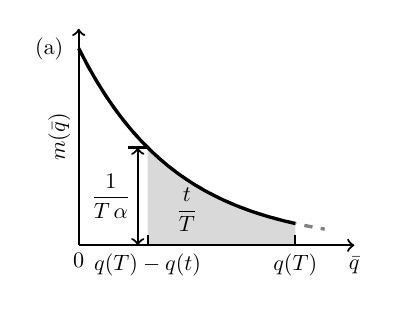
\begin{tikzpicture}[thick, scale=1.25, every node/.style={scale=0.8}]
    \node [] at (-0.3, 2.0) {(a)};
    % distribution
    \draw[domain=0:2.5, variable=\x, dashed, gray, very thick]
      plot({\x}, {2*exp(-\x)});

    % shade
    \fill [gray!30!white, domain=0.7:2.2, variable=\x]
      (0.7, 0) --
      plot ({\x}, {2*exp(-\x)})
      -- (2.2, 0) -- cycle;

    % thick curve
    \draw[domain=0:2.2, variable=\x, very thick]
      plot({\x}, {2*exp(-\x)});

    % label for the shaded area
    \node[] at (1.1, 0.36) {$\dfrac{t}{T}$};

    \draw[<->] (0.6, 0)  --
               node[left, inner sep=1mm]
               {$\dfrac{1}{T \, \alpha}$}
               (0.6, 0.99317);
    % label for the ordinate
    %\node[fill=white] at (0.4, 0.7) {$\dfrac{1}{Ta}$};

    \draw[] (0.5, 0.99317) -- (0.7, 0.99317);
    \draw[->] (0, 0) -- (2.8, 0);
    \node[] at (2.8, -0.2) {$\bar q$};
    \draw[->] (0, 0) -- node[above, rotate=90] {$m(\bar q)$} (0, 2.2);

    % xtics
    \draw[] (0.0, 0.1) -- (0.0, 0.0) node[below] {$0$};
    \draw[] (0.7, 0.1) -- (0.7, 0.0) node[below] {$q(T) - q(t)$};
    \draw[] (2.2, 0.1) -- (2.2, 0.0) node[below] {$q(T)$};
  \end{tikzpicture}
%
  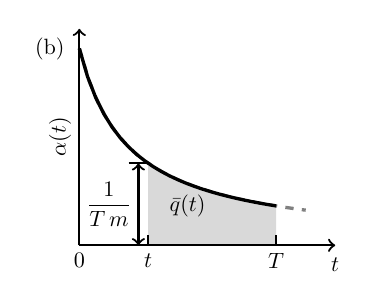
\begin{tikzpicture}[thick, scale=1.25, every node/.style={scale=0.8}]
    \node [] at (-0.3, 2.0) {(b)};
    % distribution
    \draw[domain=0:2.3, variable=\x, dashed, gray, very thick]
      plot({\x}, {1/(\x+0.5)});

    % shade
    \fill [gray!30!white, domain=0.7:2.0, variable=\x]
      (0.7, 0) --
      plot ({\x}, {1/(\x+0.5)})
      -- (2.0, 0) -- cycle;

    % thick curve
    \draw[domain=0:2.0, variable=\x, very thick]
      plot({\x}, {1/(\x+0.5)});

    % label for the shaded area
    \node[] at (1.1, 0.40) {$\bar q(t)$};

    \draw[<->] (0.6, 0)  --
               node[left, inner sep=1mm]
               {$\dfrac{1}{T \, m}$}
               (0.6, 0.83333);
    % label for the ordinate
    %\node[fill=white] at (0.4, 0.7) {$\dfrac{1}{Ta}$};

    \draw[] (0.5, 0.83333) -- (0.7, 0.83333);
    \draw[->] (0, 0) -- (2.6, 0);
    \node[] at (2.6, -0.2) {$t$};
    \draw[->] (0, 0) -- node[above, rotate=90] {$\alpha(t)$} (0, 2.2);

    % xtics
    \draw[] (0.0, 0.1) -- (0.0, 0.0) node[below] {$0$};
    \draw[] (0.7, 0.1) -- (0.7, 0.0) node[below] {$t$};
    \draw[] (2.0, 0.1) -- (2.0, 0.0) node[below] {$T$};
  \end{tikzpicture}
  \caption{
    \label{fig:massq}
    (a) Geometric construction of the optimal schedule,
    $\alpha(t)$,
    from the normalized mass distribution,
    $m(\bar q)$.
    %
    (b) Inverse construction of $m(\bar q)$
    from the optimal schedule $\alpha(t)$.
    %
    \note{
      The figure was produced by \texttt{tikz}.
    }%
  }
\end{center}
\end{figure}

We may consider the schedule, $\alpha(t)$,
as a variable transformation of
the mass distribution, $m(\bar q)$.
%much like the Legendre transform.
%
If we define
$\bar q^* \equiv \bar q/q(T)$
and $t^* \equiv t/T$
such that both are limited to the interval $[0, 1]$,
as well as
\begin{align*}
  m^*       &\equiv q(T) \, m(\bar q) = -\frac{ dt^* } { d\bar q^* },
  \\
  \alpha^*  &\equiv \frac{T}{q(T)} \, \alpha(t) = -\frac{ d\bar q^* } { dt^* },
\end{align*}
then it is clear that
both $m^*(\bar q^*)$ and $\alpha^*(t^*)$
can describe the differential relation
between $\bar q^*$ and $t^*$,
but with the natural variables
being $\bar q^*$ and $t^*$, respectively.
%
Further, the transformation is an involution:
if we apply the same transform on $\alpha^*(t^*)$
we would recover $m^*(\bar q^*)$,
as shown in Fig. \ref{fig:massq}.
%
A few examples are shown in Table \ref{tab:m_and_a}.
%
For example, in the single-bin scheme,
the mass distribution is a single exponential decay,
and we would have the inverse-time schedule.
%
On the other hand,
if the mass distribution is inversely proportional to $\bar q$,
which is approximately true for the Gaussian updating scheme
at large $\bar q$,\footnote{If
  the magnitude of the eigenvalues, $\lambda_k$'s,
  span a wide range, then for a large $\bar q$,
  the sum in Eq. \eqref{eq:mass_func} will be dominated by
  the largest term, where $\lambda_k \approx 1/\bar q$,
  and $M(\bar q) \approx \sqrt{\Gamma_k}/\bar q$.
  }
  %
then we would have an exponentially decaying schedule.

\begin{table}[h]
  \caption{\label{tab:m_and_a}
    Examples of the variable transformation between the
    reduced schedule, $\alpha^*(t^*)$,
    and the reduced mass distribution, $m^*(\bar q^*)$,
    as defined in Eqs. \eqref{eq:mQ_invTa}
    and \eqref{eq:intmQ_tT}.
  }
  \setlength{\tabcolsep}{2pt} % spacing between columns
  \renewcommand\arraystretch{2.0} % spacing between rows
  \begin{tabular} { c c c }
    \hline
    $m^*(\bar q^*)$ &
    $\alpha^*(t^*)$ &
    $\bar q^*(t^*)$
    \\
    \hline
    $\dfrac{1}{\gamma \, ({\bar q}^* + s_\gamma) }$ &
    $(1 + s_\gamma) \, \gamma \, e^{-\gamma \, t^*}$ &
    $(1 + s_\gamma) \, e^{-\gamma \, t^*} - s_\gamma$
    \\
    $(1+ s_\gamma) \, \gamma \, e^{-\gamma \, {\bar q}^*}$ &
    $\dfrac{1}{ \gamma \, (t^* + s_\gamma) }$ &
    $\dfrac{1}{\gamma} \ln\left(\dfrac{1 + s_\gamma}{t^* + s_\gamma} \right)$
    \\
    $\dfrac{c \, a}{\left( {\bar q}^* + q^*_0 \right)^{a+1}}$ &
    $\dfrac{c^{1/a} \, (1/a)}{\left( t^* + t^*_0 \right)^{(1/a)+1}}$ &
    %$\left( \dfrac{c}{t^* + t^*_0} \right)^{1/a} - q^*_0$
    $q^*_0 \left[\left( \dfrac{1+t^*_0}{t^* + t^*_0} \right)^{1/a} - 1\right]$
    %$\,\begin{aligned}
    %  &a, q^*_0 > 0, \\
    %  &\frac{1}{t^*_0} \equiv \left(1+\frac{1}{q^*_0}\right)^a - 1, \\
    %  &c \equiv {q^*_0}^a(t^*_0 + 1)
    %\end{aligned}$
    \\
    \hline
    \multicolumn{3}{p{8cm}}{
    Here,
    $\gamma > 0$,
    and we have defined
    $s_\gamma \equiv 1/(e^\gamma - 1)$,
    ${t^*_0}^{-1} \equiv \left(1+{q^*_0}^{-1}\right)^a - 1$,
    and
    $c \equiv {q^*_0}^a(1 + t^*_0)$.
    } \\
    \hline
  \end{tabular}
\end{table}








\subsubsection{\label{sec:optinitalpha}
  Optimal initial updating magnitude
}


We now determine the optimal value of $q(T)$
that minimizes the total error defined in Eq. \eqref{eq:error_tot}.
%
We will consider simulations in which
the system is initially equilibrated at a
constant updating magnitude, $a_0$.
%
From Eqs. \eqref{eq:error_res}, \eqref{eq:xt2_eql1},
and \eqref{eq:error_asym2},
we find that
the optimal $q(T)$ satisfies
%
\begin{align}
  \mathcal Y\bigl( q(T) \bigr)
  &\equiv
  \frac{ M\bigl( q(T) \bigr) } { T }
    \int_0^{q(T)} M(q') \, d q'
  -\frac{a_0}{2} \, M^2\bigl( q(T) \bigr)
  \notag \\
  &
  -\sum_{k = 1}^{n-1}
  \lambda_k \, \epsilon_k \, e^{-2\lambda_k \, q(T)}
  =0
  .
\label{eq:opt_qT}
\end{align}
%
%\begin{align}
%  m\bigl( q(T) \bigr)
%  +
%  \frac{2}{a_0 \, C_M \, M\bigl( q(T) \bigr)}
%  \sum_{k = 1}^{n-1}
%  \lambda_k \, \tilde u_k^2 \,
%  e^{-2 \, \lambda_k \, [a_0 \, T_0 + q(T)] }
%  \\=
%  \frac{1} { T \, (a_0 / 2) }
%  .
%\label{eq:opt_qT}
%\end{align}
%
\note{Let $q_T \equiv q(T)$,
$$
\begin{aligned}
  \frac{
    \partial \Err_R(T)
  }
  {
    \partial q_T
  }
  &=
  -a_0 \, M^2(q_T)
  -2
  \sum_{k=1}^{n-1} \lambda_k \,
  \tilde u_k^2 e^{-2 \, \lambda_k \, (a_0 \, T_0 + q_T)}
  ,
  \\
  \frac{
    \partial \Err_A(T)
  }
  {
    \partial q_T
  }
  &=
  \frac 2 T \,
  M(q_T) \,
  \int_0^{ q_T } M(q) \, dq
  =
  \frac{ 2 \, C_M } { T } \, M(q_T)
  .
\end{aligned}
$$
Then solve $\partial (\Err_R + \Err_A) / \partial Q_c = 0$.
}
%
We can rewrite the condition in terms of
the initial updating magnitude by Eq. \eqref{eq:mQ_invTa},
\begin{align}
  \alpha(0)
  =
  \frac{1}{T \, m\bigl( q(T) \bigr) }
  =
  \frac{ a_0 } { 2 }
  +
  \sum_{k = 1}^{n-1}
  \frac{
    \lambda_k \, \epsilon_k \, e^{-2\lambda_k \, q(T)}
  }{M^2\bigl( q(T) \bigr)}
  .
  \label{eq:opt_alpha0}
\end{align}
%
If the initial bias, $\epsilon_k$, is negligible,
which is typically true if no eigenvalue is close to $0$,
then
%
\begin{equation}
  \alpha( t = 0 )
  \approx
  \frac{ a_0 }
       { 2 }
  ,
\label{eq:half_alpha0}
\end{equation}
%
i.e. the optimal initial updating magnitude
is half of the equilibrium value.\footnote{This factor, $1/2$,
happens to coincide with the
recommended reduction factor of the updating magnitude
at stage transitions
in the original WL algorithm\cite{
wang2001, wang2001pre}.
}



\subsubsection{\label{sec:band-matrix}
Homogeneous updating schemes}



Many commonly-used updating schemes,
such as the Gaussian updating scheme
used in metadynamics,
can be characterized by a rigid window
centered on the current bin.
%
For these translationally invariant or homogeneous
schemes, the eigenvalues can be readily found
from the window function ($\mu_0, \mu_1, \dots, \mu_b$)
as a cosine transform,
%
\begin{equation}
  \lambda_k
  =
  \mu_0
  +
  2 \,
  \sum_{ i = 1 }^b
  \mu_i
  \cos\left(
  \frac{ k \, i \, 2 \, \pi }
       {      g \, n        }
  \right)
  ,
  \label{eq:wband_eigenvalue}
\end{equation}
%
where $g = 1$ here for the periodic variable,
or $2$ for a non-periodic one
(cf. Appendix \ref{sec:more_wband}).
%
For the Gaussian updating scheme,
we have\cite{bussi2006}
\begin{align}
  \lambda_k
  =
  \exp\left[
        -\frac 1 2
        \left(
         \frac{ 2 \, \pi \, k \, \sigma_z }
              { g \, \Delta z  }
        \right)^2
      \right]
  ,
%\notag
\label{eq:lambda_Gaussian}
\end{align}
where $\sigma_z$ and $\Delta z = z_{\max} - z_{\min}$
are the width of the Gaussian and span
in the original collective variable, $z$,
respectively.


\subsubsection{\label{sec:procedure}
Procedure of computing the optimal schedule and error
}


Based on the above results,
we now give a procedure of computing
the optimal schedule and the error
for a given adaptive FDS simulation.
%
Basically, we need to extract
$\lambda_k$'s and $\Gamma_k$'s
from the given system and updating scheme (input),
and then apply them to Eq. \eqref{eq:q_opt}
for the schedule,
as shown in Fig. \ref{fig:vardep}.
%
While the updating scheme alone
determines $\lambda_k$'s,
$\Gamma_k$'s depend also on the system
and the underlying sampling process.
%
We have

\begin{figure}[h]
\begin{singlespace}
  \fontsize{10pt}{\baselineskip}
  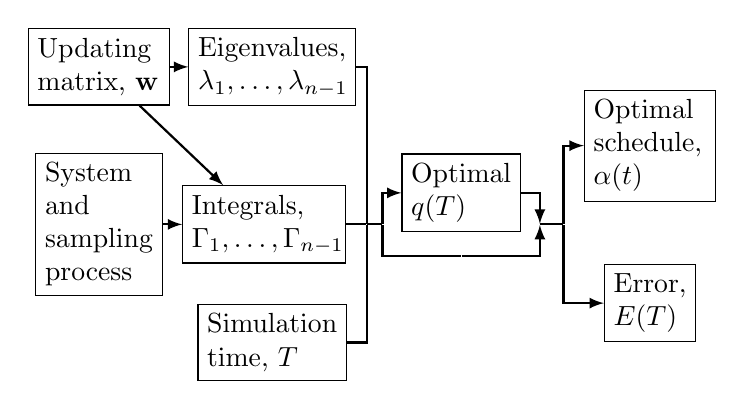
\begin{tikzpicture}
  \node[draw, text width={width("Updating ")}]
    (w) at (0, 3) {Updating \\matrix, $\mathbf w$};

  \node[draw, text width={width("sampling")}]
    (sys) at (0, 1) {System\\and\\sampling\\process};

  \node[draw, text width={width("Eigenvalues,")}]
    (lambda) at (2.2, 3) {Eigenvalues,\\$\lambda_1, \dots, \lambda_{n-1}$};

  \node[draw, text width={width("Integrals, iii")}]
    (Gamma) at (2.1, 1) {Integrals, \\$\Gamma_1, \dots, \Gamma_{n-1}$};

  \node[draw, text width={width("Simulation")}]
    (T) at (2.2, -0.5) {Simulation\\time, $T$};

  \node[draw, text width={width("Optimal")}]
    (qT) at (4.6, 1.4) {Optimal\\ $q(T)$};

  \node[draw, text width={width("Schedule,")}]
    (alpha) at (7, 2) {Optimal schedule,\\ $\alpha(t)$};

    \node[draw, text width={width("Error,")}]
    (err) at (7, 0) {Error, $\Err(T)$};

  \node[inner sep=0, minimum size=0] (M1) at (3.4, 1) {};

  \node[inner sep=0, minimum size=0] (N1) at (5.9, 1) {};

  \node[inner sep=0, minimum size=0] (R1) at (3.6, 1) {};
  \node[inner sep=0, minimum size=0] (R2) at (4.6, 0.6) {};
  \node[inner sep=0, minimum size=0] (R3) at (5.6, 1) {};

  \draw[->, >=latex, thick]
    (w) edge (lambda)
    (w) edge (Gamma)
    (sys) edge (Gamma);

  \draw[->, >=latex, thick]
    (lambda) -| (M1)
    (Gamma)  -- (M1)
    (T)      -| (M1)
    (M1)     -- (R1)
    (R1)     |- (qT);

  \draw[->, >=latex, thick]
    (qT)     -| (R3);

  \draw[->, >=latex, thick]
    (R3) -- (N1) |- (alpha);

  \draw[->, >=latex, thick]
    (N1) |- (err);

  \draw[->, >=latex, thick]
    %(M1) edge[bend left=70] (N1);
    (R1) |- (R2) -| (R3);
\end{tikzpicture}
\end{singlespace}
\caption{
  \label{fig:vardep}
  Dependence of variables in computing
  the optimal schedule and the error.
}
\end{figure}




\begin{enumerate}

\item
Compute the eigenvalues, $\lambda_k$'s
from the updating matrix, $\mathbf w$,
or from Eq. \eqref{eq:wband_eigenvalue}
for a homogeneous updating scheme.
%
Note that
no eigenvalue can be negative for the updating scheme to be stable.

\item \label{step:prerun}
Run a preliminary adaptive FDS simulation
under constant updating magnitude, $a_0$.
%
\note{The updating magnitude should be sufficiently small
  such that the resulting error is no greater than
  multiple of $1.0$.}

\item \label{step:Gamma}
Estimate $\Gamma_k$'s from Eq. \eqref{eq:varXt}
(cf. Appendix \ref{sec:Gamma_measure})
as well as the initial bias $\epsilon_k$.\footnote{The
  value of $\tilde u_k$ can be estimated
  from the histogram-corrected bias potential
  by Eq. \eqref{eq:uhatav},
  although it can overestimate
  $\epsilon_k$ for large-$k$ modes.
}

\item \label{step:qT}
Compute the optimal value of $q(T)$ by solving Eq. \eqref{eq:opt_qT}.
%
We implemented a variant of the Newton-Raphson method\cite{press3rd}
with the bisection method\cite{press3rd}
as a fallback.\footnote{
The equation was solved for $\ln q(T)$
to avoid negative values of $q(T)$,
and we imposed a lower bound,
$\bigl|\mathcal Y\bigl(q(T)\bigr)/q(T)\bigr|$, for
$\mathcal Y'\bigl(q(T)\bigr)$
in computing its change.
}
The initial value is set to $q(T) = \ln(1+T\,a_0/2)$.
%
%Since $m(\bar q)$ is a decreasing function of $\bar q$,
%we can start from an interval $[Q_L, Q_R]$
%that satisfies $m(Q_L) > 2/(T\,a_0) > m(Q_R)$
%(e.g. we can choose $Q_L = 0$,
%  and repeatedly double $Q_R$ until
%  the latter inequality is satisfied).
%%
%We can then iteratively refine the interval
%by substituting $Q_M = (Q_L + Q_R)/2$
%for either $Q_L$ and $Q_R$,
%depending on the sign of $m(Q_M) - 2/(T \, a_0)$,
%until the width of the interval is less than
%the desired precision,
%%
%and set $q(T)$ to $Q_M$.

\item \label{step:alpha}
Compute the optimal schedule by
  numerically integrating Eqs. \eqref{eq:q_opt} and \eqref{eq:mint}.
%
To handle Gaussian updating schemes more effectively,
  we have chosen the $\mathcal N+1$ grid points over $[0, q(T)]$ to be given by
  $q_{[i]} = \bigl(q(T) + 1\bigr) - \bigl(q(T)+1\bigr)^{1-i/\mathcal N}$,
  where $i = 0, \dots, \mathcal N$,\footnote{For
    a mass distribution, $m(\bar q)$, that is
    inversely proportional to $\bar q$,
    this grid would make the integral,
    or the difference, $t_{[i+1]} - t_{[i]}$,
    roughly a constant.}
  and we chose $\mathcal N=20000$.
%
The curve $q(t)$ is then integrated
  using the trapezoidal rule\cite{press3rd},
  resulting in a list of values, $\bigl(q_{[i]}, t_{[i]} \bigr)$.
%
We then compute the updating magnitude by numerical differentiation:
  $\alpha_i = (1 - e^{-\lambda_1 \, \hat \alpha_i})/\lambda_1$\footnote{This
    discretization follows from runtime average interpretation
    discussed in Appendix \ref{sec:equilerr}.}
  and
  $\hat \alpha_i \equiv (q_{[i+1]} - q_{[i-1]}) / (t_{[i+1]} - t_{[i-1]})$,
  with
  $q_{[ -1]} \equiv 0$,
  $q_{[N+1]} \equiv q(T)$,
  $t_{[ -1]} \equiv 0$, and
  $t_{[N+1]} \equiv T$.
%
The resulting values of $(t_{[i]}, \alpha_{[i]})$
  can be linearly interpolated
  to get the updating magnitude, $\alpha(t)$, at any simulation time, $t$.


\item
  Compute the total error $\Err(T)$ from
Eqs. \eqref{eq:error_tot},
  \eqref{eq:error_res},
  \eqref{eq:xt2_eql1},
  and
  \eqref{eq:error_asym2}.

\end{enumerate}

The above procedure is not always necessary.
%
As shown below, for a class of bandpass updating schemes,
  which resemble the Gaussian updating schemes,
  the asymptotically optimal schedule
  is simply given by the inverse-time schedule, Eq. \eqref{eq:alpha_invt1}.
%
%For these updating schemes,
%  the preliminary run with a constant updating magnitude
%  can be replaced by the WL-style stagewise reduction
%  until the updating magnitude falls under
%  the value given the inverse-time prescription\cite{
%    belardinelli2007, *belardinelli2007jcp, *belardinelli2008, *belardinelli2016}.



\subsection{\label{sec:cmpschemes}
Comparison of updating schemes}


Now that we can compute the optimal schedule
for a given updating scheme,
we will turn to the problem of finding
optimal updating schemes.


\subsubsection{\label{sec:optWL}
Asymptotic optimality of the single-bin scheme}



We will first show
that the single-bin scheme is asymptotically optimal.
%
Consider a class of $\mathbf w$ matrices
sharing the same set of eigenvectors,
hence the same $\Gamma_k$'s,
but with different positive eigenvalues,
$\lambda_k$'s.
%
Using the Cauchy-Schwarz inequality, we have,
for any set of nonnegative numbers, $c_k$'s\footnote{This
inequality follows from the nonnegativity of
the quadratic polynomial,
$$
\int_0^T
  dt \sum_{k = 1}^{n-1} \Gamma_k \,
    \left( {\dot \vartheta}_k \, \chi - c_k \right)^2
  \equiv
  A_2 \, \chi^2 + A_1 \, \chi + A_0
  ,
$$
which implies a nonpositive discriminant,
$A_1^2 - 4 \, A_0 \, A_2$.}
%
%
\begin{align}
&
\left(
  \int_0^T dt
    \sum_{k = 1}^{n-1}
      \Gamma_k \, {\dot \vartheta}_k^2\bigl( q(t) \bigr)
\right)
%
\left(
  \int_0^T dt
    \sum_{k = 1}^{n-1}
      \Gamma_k \, c_k^2
\right)
%
\notag
\\
&
\qquad \qquad
\ge
\left(
  \int_0^T dt
    \sum_{k = 1}^{n-1}
      \Gamma_k \, c_k \, {\dot \vartheta}_k \, \bigl( q(t) \bigr)
\right)^2
\notag
\\
&
\qquad \qquad
=
\left(
  \sum_{k = 1}^{n-1} \Gamma_k \, c_k
    \left[
      1 - e^{ -\lambda_k \, q(T) }
    \right]
\right)^2.
\notag
%\label{eq:CSineq}
\end{align}
%
Note that the last expression %of Eq. \eqref{eq:CSineq}
depends on the curve, $q(t)$ ($0 < t < T$),
only through the endpoint value, $q(T)$,
which is fixed in the variational process.
%
Thus, the inequality sets a lower bound
for the asymptotic error $\Err_A(T)$
given in Eq. \eqref{eq:error_asym}.
%
The equality is achieved
if $\dot \vartheta_k\left( q(t) \right) = c_k$
for all $k > 0$ at any $t$,
up to a multiplicative factor.
%
Solving these equations yields
a set of identical eigenvalues,
$\lambda_1 = \cdots = \lambda_{n-1}$
and identical $c_k$'s.

Since an updating matrix
with identical eigenvalues\footnote{Since
  the eigenmode of $k = 0$ represents
  a uniform shift of the bias potential,
  we can freely set $\lambda_0$ to be
  the same as $\lambda_1$
  without changing the nature of
  the updating scheme.}
is a multiple of the identity matrix,
%
if the eigenvalues are set to $1$,
we recover the single-bin scheme.
%
This means that the single-bin scheme is most efficient
in error reduction in the asymptotic limit.
%
In particular,
with $\vartheta_k = (t+t_0)/(T+t_0)$,
we can readily recover the optimal schedule,
Eq. \eqref{eq:alpha_invt1}, with
the asymptotic error being
$\Err_A(T) = T / (T + t_0)^2 \sum_{ k = 1 }^{n-1} \Gamma_k$,
%
%\begin{align}
%  \Err_A(T)
%  =
%  \frac{       T     }
%       { (T + t_0)^2 }
%  \sum_{ k = 1 }^{n-1}
%    \Gamma_k
%  ,
%\end{align}
%
which is identical to Eq. \eqref{eq:EA_sbin1}
if we notice [cf. Eq. \eqref{eq:parseval}]
%
%where we have used
%
\begin{align}
  \sum_{k=1}^{n-1} \Gamma_k
  &=
  \sum_{t=-\infty}^\infty \sum_{k=1}^{n-1}
  \bigl\langle {\tilde \zeta}_k(t) \, {\tilde \zeta}_k(0) \bigr\rangle
  \notag
  \\
  &=
  \sum_{t=-\infty}^\infty \sum_{i=1}^n
  \rho_i \bigl\langle \zeta_{*i}(t) \, \zeta_{*i}(0) \bigr\rangle
  = \sum_{i=1}^n \rho_i \, G_i = \Gamma
  .
  \notag
  %\label{eq:Gamma_G_sum}
\end{align}
%%




\subsubsection{\label{sec:bandpass}
Bandpass updating schemes}


We can generalize
the single-bin scheme to a class of
perfect (brick-wall) \emph{bandpass} updating schemes
that completely eliminates certain short-wavelength eigenmodes,
which are typically local noise.
%
A bandpass updating scheme is essentially
the single-bin updating scheme
followed by a perfect filter
for the designated noise modes,
and zero eigenvalues are assigned to these modes.
%
For example,
by assuming
that the PMF is so smooth
that it can be represented by the first $K$
modes,\footnote{As an estimate of error,
  we note that truncating a linear or quadratic function
  at mode $K$ (for a non-periodic variable)
  results in an error roughly proportional to
  $|\max_i u_i - \min_i u_i|^2/K^3$.}
we demand
%
\begin{equation}
  \lambda_1 = \cdots = \lambda_{K-1} = 1,
  \mathrm{\; and \;}
  \lambda_K = \cdots = \lambda_{n-1} = 0.
  \label{eq:lambda_bandpass}
\end{equation}
%
%Then, the updating matrix is, according to
%Eq. \eqref{eq:w_from_phi},
%%
%$$w_{ij} = \frac{1}{\rho_i} \sum_{k=0}^{K-1} \phi_{ki} \, \phi_{kj}.$$
%%
The asymptotic error is then
$\Err_A(T) = \sum_{ k = 1 }^{ K - 1 } \Gamma_k T/(T + t_0)^2$,
which is less than that from Eq. \eqref{eq:EA_sbin1}.
%
The optimal schedule of these schemes
remains the inverse-time schedule
given by Eq. \eqref{eq:alpha_invt1}
with $t_0$ given by Eq. \eqref{eq:t0_sbin}.
%
%The asymptotic error is given by
%%
%\begin{equation}
%  \Err_A(T)
%  =
%  \frac{   T     }
%       { (T + t_0)^2 }
%  \sum_{ k = 1 }^{ K - 1 }
%    \Gamma_k
%  ,
%  \notag
%  %\label{eq:error_sinc}
%\end{equation}
%%
%as a generalization of Eq. \eqref{eq:Emin_sbin}
%for the single-bin updating scheme.
%

Since bandpass updating schemes
straightforward generalizations of
the single-bin updating scheme,
we can also borrow the WL algorithm
to control the updating magnitude
in initial stages of the simulation.
%
However, the histogram fluctuation should
be limited to first $K$ modes,
as the bandpass updating scheme
only partially flattens these histogram
modes (cf. Appendix \ref{sec:hfluc}).


In addition to the application to homogeneous updating schemes
(Appendix \ref{sec:homo_bandpass}),
bandpass updating schemes can also be applied to
a continuous variable, $z$,\footnote{
  In the transition to a continuous variable,
  we will map
  $\rho_i$ to $\rho(z) \, \delta z$,
  $\phi_{ki}$ to $\phi_k(z) \, \delta z$,
  $w_{ij}$ to $w(z, z') \, \delta z$, etc.}
with the eigenmodes derived from orthogonal polynomials, $R_k(z)$,
that satisfy
\begin{align*}
  \int R_k(z) \, R_{k'}(z) \, \rho(z) \, d z = \delta_{k, k'}
  .
\end{align*}
%
With $\phi_k(z) = R_k(z) \, \rho(z)$,
we can readily satisfy Eqs. \eqref{eq:eig_orthonormal_cols}-\eqref{eq:ortho0},
and construct the updating matrix by
Eqs. \eqref{eq:w_from_phi} and \eqref{eq:lambda_bandpass} as
\begin{align*}
  w(z, z')
  =
  \sum_{k=1}^{K-1} \frac{ \phi_k(z) \, \phi_k(z') } { \rho(z) }
  = \sum_{k=1}^{K-1} R_k(z) \, R_k(z') \, \rho(z'),
\end{align*}
%
where we have dropped the $k=0$ mode
that corresponds to a uniform shift
of the bias potential.
%
The resulting bias potential
assumes a polynomial form
and can be written as a superposition
$u(z, t) = \sum_{k=1}^{K-1} c_k(t) \, R_k(z)$,
with the coefficients updated as, according to Eq. \eqref{eq:mbin_update},
\begin{equation}
  c_k(t+1) = c_k(t) + \alpha(t) \, R_k\bigl( z(t) \bigr)
  .
  \label{eq:ckupdate}
\end{equation}


For example,
to sample a flat distribution, $\rho(z)$,
over $[z_c - \Delta z/2, z_c + \Delta z/2]$,
we can use the Legendre polynomials\cite{arfken},
and with $K = 2$,
the bias potential contains only a linear mode for
$R_1(z) = 2 \sqrt{3} \, (z - z_c)/\Delta z$,
with its coefficient, $c_1$, updated according to
the difference between the average of $z$
and the center $z_c$.
%
We thus recover the Langfeld-Lucini-Rago (LLR)
algorithm\cite{langfeld2012},
and the inverse-time schedule
was recommended for optimal convergence of $c_1$\cite{pellegrini2014}.

Alternatively,
to sample a Gaussian distribution
centered at $z_c$ with width $\sigma_z$
we can use the Hermite polynomials\cite{arfken}.
%
With $K = 3$, the bias potential is quadratic
and is a linear combination of
$R_1(z) = (z - z_c)/\sigma_z$
and
$R_2(z) = \bigl[(z - z_c)^2 - \sigma_z^2\bigr] /\left(\sqrt 2 \, \sigma_z^2\right)$.
%
Note that quadratic bias potentials are commonly employed
in umbrella sampling (see e.g. Ref. \cite{zhu2012})
and the method of Gaussian ensemble\cite{hetherington1987,
*challa1988, *costeniuc2006, neuhaus2006, *neuhaus2007},
which is helpful in overcoming barriers
in first-order phase transitions.
%
By Eq. \eqref{eq:ckupdate},
$c_1$ and $c_2$ are updated
according to the first and second
central moments of $z$, respectively.
%
Below we will refer to this application
as adaptive Gaussian umbrella sampling.

The use of a polynomial basis makes
the bias potential smooth and differentiable,
and hence suitable for MD applications.\cite{zhu2012}
%
However,
the distribution, $\rho_i$,
has to be sufficiently narrow
because of the limited number of modes
in controlling the moments.
%
We can nonetheless sample a wider range
by constructing a mixture\cite{shirts2017}
or an expanded ensemble
from a superposition of multiple Gaussian umbrellas
centered at different places via
the frameworks of
parallel\cite{swendsen1986,
  *geyer1991, *hukushima1996, *hansmann1997, *sugita1999, *earl2005}
and/or simulated tempering\cite{marinari1992,
  *lyubartsev1992, li2007,
  park2007, *nguyen2013, *zhang2015st}.
%
While the mutual exchange probability
can be readily derived in the former
framework\cite{neuhaus2006, *neuhaus2007},
the transition probability in the latter case
requires estimation of the partition function
of the Gaussian ensemble
$Z \equiv \int e^{-\beta \, \mathcal U(\mathbf x)-u(z(\mathbf x),t)} \, d\mathbf x$,
where
$\beta$ is the inverse temperature,
$\mathcal U(\mathbf x)$ is the unbiased potential energy
as a function of molecular coordinates, $\mathbf x$,
and $z$ has also been written as a function of $\mathbf x$.
%
The transition probability from
the $i$th umbrella to the $j$th is given by
\begin{align*}
A(i\to j) =
\min\left\{1,
  \frac{Z^{(i)}}{Z^{(j)}}
  \exp\left[u^{(i)}\bigl( z(t) \bigr)
   - u^{(j)}\bigl( z(t) \bigr) \right]
  \right\}
  ,
\end{align*}
where $z(t)$ is the current value of $z$.
%
While the asymptotic updating magnitude
would be given by the inverse-time formula,
we can employ the WL strategy early in simulation
to control the updating magnitude in stages
with the histogram fluctuation
redefined by Eq. \eqref{eq:maxFk}
(including the intra-umbrella and inter-umbrella
components).
%
The weighted histogram analysis method
(WHAM)\cite{ferrenberg1988, *ferrenberg1989,
*kumar1992, *roux1995, *bartels1997, *souaille2001,
*kobrak2003, *gallicchio2005, *chodera2007,
*fenwick2008, *kim2011, *shirts2008,
zhu2012, newman, frenkel},
can be used to recover the unbiased distribution
after simulation.
%

\note{The
  following method appeared to have some stability issues,
  so we switched back to the double-WL approach,
  which hopefully is stable.
  %
  The reason of instability might be
  that the inter-umbrella fluctuation
  and the intra-umbrella fluctuation are some coupled.
  So the updating magnitude cannot be adjusted individually
  for the each umbrella.
  %
  Following the method for weight determination
  in simulated tempering\cite{park2007,
  *nguyen2013, *zhang2015st},
  we can estimate $Z^{(j)}/Z^{(i)}$
  for a neighboring pair, $(i, j)$, as
  %
  \begin{align*}
    &\ln\frac{ Z^{(j)} }{ Z^{(i)} }
    \approx
    \ln\frac{ \sigma_z^{(j)} }{ \sigma_z^{(i)} }
    +
    \frac{ \Delta z_c } { 2 }
    \left(
      \frac{ c_1^{(i)} } { \sigma_z^{(i) 2} }
      +
      \frac{ c_1^{(j)} } { \sigma_z^{(j) 2} }
    \right)
    +
    \frac{ c_2^{(j)} - c_2^{(i)} } { \sqrt 2 }
    \\
    &-
    \left(
      \frac{ \sqrt 2 \, c_2^{(j)} - 1 }
           { 2 \, \sigma_z^{(j)} }
      -
      \frac{ \sqrt 2 \, c_2^{(i)} - 1 }
           { 2 \, \sigma_z^{(i)} }
    \right)
    \left(
      \frac{ \Delta z_c^{2} } { 6 }
      +
      \frac{ \sigma_z^{(i) 2} + \sigma_z^{(j) 2} } { 2 }
    \right)
    ,
  \end{align*}
  %
  where
  $\Delta z_c \equiv z_c^{(j)} - z_c^{(i)}$.
  For equal width, we have
  \begin{align*}
    \ln\frac{ Z^{(j)} }{ Z^{(i)} }
    \approx
    \frac{ \Delta z_c \, ( c_1^{(i)} + c_1^{(j)} ) } { 2 \, \sigma_z }
    -
    \left(
      \frac{ c_2^{(j)} - c_2^{(i)} }
           { 6 \sqrt 2 }
    \right)
    \left(
      \frac{ \Delta z_c^{2} } { \sigma_z^2 }
    \right)
    .
  \end{align*}
}



\section{\label{sec:results}
Numerical results}



\subsection{\label{sec:lj}
Comparison of updating schemes on a Lennard-Jones fluid}


Our test system is a Lennard-Jones (LJ) fluid of $100$ particles,
and we wish to compute the PMF along the distance of two special particles, $r$.
%
The two special particles are mutually non-interacting
but they interact normally with other particles,\footnote{They
were placed on an axis parallel to a side of the cubic box}
and the intrinsic distribution, $p(r)$, is
the cavity distribution function, $y(r)$\cite{hansen}.
%
We will assume reduced units in this calculation.
%
The reference bias potential was pre-calculated from a long simulation.

We used the Metropolis algorithm\cite{frenkel, metropolis1953}
for configuration sampling.
%
Each step consists of
one MC trial for displacing one of the two special particles,
and another four trials for displacing the other particles.
%
In each trial, the displacement along each dimension is uniform,
with the size given by $0.1/\varrho^*$
to ensure the acceptance ratio is around 50\%,
where $\varrho^*$ is the reduced number density.


The PMF was calculated from $r = 0$ to half of the box size
(also the cutoff distance of the potential)
on a grid of size $\delta r = 0.01$ in reduced units.
%
Two densities were tried, $\varrho^* = 0.1$ and $0.8$,
and the numbers of bins were $n = 500$ and $250$, respectively.
%
The reduced temperature was $T^* = 3$.
%
We tested the single-bin, Gaussian, and bandpass updating schemes.
%
Each simulation started with an ``equilibration'' phase
of $10^7$ steps under constant updating magnitude,
$a_0 = 10^{-4}$,\footnote{The equivalent $\ln f = n \, a_0$ for the WL algorithm
was $0.05$ and $0.025$, respectively.}
followed by a production phase of another $10^7$ steps
with updating magnitude given by
either the inverse-time or optimal schedule.
%
We repeated each simulation multiple times
and report the average.
%
To make sure the same schedule for multiple runs under the same condition,
the optimal schedule was pre-computed from a set of fixed values of
$\Gamma_k$ and $\epsilon_k$,
although they can be fairly accurately estimated from the data
collected from the equilibration phase of each individual run.



As shown in Table \ref{tab:lj_error},
all updating schemes
with either the inverse-time or optimal schedule
were able to reduced
the error significantly,
and the errors roughly matched the predicted values
calculated from the pre-computed
$\Gamma_k$'s and $\epsilon_k$'s.
%
The Gaussian updating scheme produced less error than
the single-bin scheme in the $\varrho^* = 0.1$ case,
but not in the $\varrho^* = 0.8$ case.
%
The effectiveness of the Gaussian updating scheme
in the low density case
was probably because the sampling along
the collective variable was free from major barriers
and thus the histogram fluctuation largely
resulted from local noise.
%
%The optimal schedule also appeared to be more effective
%in reducing the error than the inverse-time schedule.
%%
In this case, we could further reduced the error
by using the bandpass updating scheme
(with the mode cutoff $K = 20$).
%
On the other hand, in the high-density case,
the error was dominated by the $k=1$ eigenmode
corresponding to the longest range fluctuation,
$\Gamma_1 \approx \Gamma$,
and the reduction of local noise
had little effect on the total error.


\begin{table}[h]\footnotesize
  \caption{\label{tab:lj_error}
    Error of the bias potential under
    the single-bin,
    Gaussian (labeled by the width, $\sigma$),
    and bandpass (labeled by the mode cutoff, $K$)
    updating schemes
    on the LJ system.
    %
    The numbers have been averaged over multiple runs,
    and the predicted values are shown in parentheses for comparison;
    $\Err_\mathrm{init.}$
    denotes the error
    at the end of the equilibration phase under constant magnitude;
    $\Err_\mathrm{final}$
    denotes the error at the end of the production phase under
    either the inverse-time ($1/t$) or optimal schedule (opt.).
    %
    \note{The reference values can be found
    on the second line of \texttt{verr.log}.}%
  }
  \setlength{\tabcolsep}{2pt}
  \renewcommand\arraystretch{1.4}
  \begin{tabular} { l c c c c }
    \hline
    Scheme & Sched. &
    $\Err_\mathrm{init.}$ &
    $\Err_\mathrm{final}$
    \\
    \hline
    \multicolumn{4}{c}{
      $\varrho^* = 0.1$,
      $500$ bins,
      $\Gamma_1 \approx 111$,
      $\Gamma \approx 1.1\times10^3$.
    } \\
    \hline
    single-bin & $1/t$
    & $5.7(5.7)\times10^{-2}$
    & $9.2(11.4)\times10^{-5}$
    \\
    %\hline
    $\sigma=0.1$ & $1/t$
    & $7.5(8.9)\times10^{-3}$
    & $6.8(8.2)\times10^{-5}$
    \\
    %\hline
    $\sigma=0.1$ & opt.
    & $7.5(8.9)\times10^{-3}$
    & $3.3(3.9)\times10^{-5}$
    \\
    %\hline
    $\sigma=0.2$ & $1/t$
    & $6.6(7.8)\times10^{-3}$
    & $3.9(4.8)\times10^{-5}$
    \\
    %\hline
    $\sigma=0.2$ & opt.
    & $6.7(7.8)\times10^{-3}$
    & $2.4(2.9)\times10^{-5}$
    \\
    %\hline
    $\sigma=0.5$ & $1/t$
    & $5.4(6.6)\times10^{-3}$
    & $3.3(3.8)\times10^{-5}$
    \\
    %\hline
    $\sigma=0.5$ & opt.
    & $5.8(6.6)\times10^{-3}$
    & $2.7(3.0)\times10^{-5}$
    \\
    %\hline
    $K=20$ & $1/t$
    & $8.0(8.9)\times10^{-3}$
    & $1.6(1.8)\times10^{-5}$
    \\
    \hline
    \multicolumn{4}{c}{
      $\varrho^* = 0.8$,
      $250$ bins,
      $\Gamma_1 \approx 2.0\times10^4$,
      $\Gamma \approx 2.7\times10^4$
    } \\
    \hline
    single-bin & $1/t$
    & $1.4(1.4)$
    & $3.4(2.7)\times10^{-3}$
    \\
    %\hline
    $\sigma=0.1$ & $1/t$
    & $1.3(1.3)$
    & $3.0(2.8)\times10^{-3}$
    \\
    %\hline
    $\sigma=0.1$ & opt.
    & $1.2(1.3)$
    & $3.0(2.8)\times10^{-3}$
    \\
    %\hline
    $\sigma=0.2$ & $1/t$
    & $1.3(1.2)$
    & $3.5(3.2)\times10^{-3}$
    \\
    %\hline
    $\sigma=0.2$ & opt.
    & $1.2(1.2)$
    & $3.1(2.9)\times10^{-3}$
    \\
    %\hline
    $\sigma=0.5$ & $1/t$
    & $1.0(0.9)$
    & $9.9(8.0)\times10^{-3}$
    \\
    %\hline
    $\sigma=0.5$ & opt.
    & $1.0(0.9)$
    & $5.9(5.4)\times10^{-3}$
    \\
    %\hline
    $K=20$ & $1/t$
    & $1.4(1.3)$
    & $3.1(2.7)\times10^{-3}$
    \\
    \hline
  \end{tabular}
\end{table}

For the Gaussian updating scheme,
there was an optimal width for maximum effectiveness.
%
The optimal width was $\sigma = 0.37$ for $\varrho^* = 0.1$
or $0.07$ for $\varrho^* = 0.8$,
and it also depended on the simulation length
and other parameters.
%
Although widening the Gaussian can
effectively suppress random error
from local histogram fluctuation,
it also increased the risk of including
more systematic bias in middle-range modes,
which can be difficult to remove
even with the optimal schedule.
%
This is because the rate of error reduction
is proportional to the eigenvalue, $\lambda_k$
[cf. Eq. \eqref{eq:vt_diffeq_mbin}],
which can decrease rapidly with the mode index $k$,
cf. Eq. \eqref{eq:lambda_Gaussian}.

To illustrate the mode dependence of the error,
we show in Fig. \ref{fig:lj_xerr}
the error components, $\langle \tilde v_k^2 \rangle$,
against the eigenmode index, $k$,
for the $\varrho^* = 0.1$ case
with width $\sigma = 0.2$.
%
For modes $k=10$ to $25$,
the final errors from the Gaussian updating scheme
were greater than those from the single-bin updating scheme
although the initial values were less.
%
For the Gaussian updating scheme,
the inverse-time schedule tended to
reduce the updating magnitude too quickly
leaving a hump on the error profile
for these middle-range eigenmodes.
%
The optimal schedule improved over the inverse-time schedule
and produced a flatter profile for the final error.
%
As a result, the optimal schedule usually produced
less error than the inverse-time schedule
as shown in Table \ref{tab:lj_error}.
%
Although the difference was small in the reported cases,
the gain of using the optimal schedule
would increase with the simulation length.\footnote{
  For example, for the $\varrho^* = 0.1$ case
  with width $\sigma = 0.2$,
  the predicted error of a simulation of $10^8$ steps
  was $2.5\times10^{-5}$ for the inverse-time schedule
  or $3.7\times10^{-6}$ for the optimal schedule.}

One way to overcome the systematic bias
in the Gaussian updating scheme
is to use the correction formula
based on histogram, Eq. \eqref{eq:uhatav}.
%
As shown in Fig. \ref{fig:lj_xerr},
even for the simulation using the non-optimal $1/t$ schedule,
the correction was able to reproduce
the flatter profile seen in the single-bin case.
%
However, this correction also introduced
some local noise in the large $k$ modes,
and it would be best used as a post-simulation
analysis tool for simulations
with detectable residual bias.
%
For example, for the simulation in the $\varrho^* = 0.8$ case
with $\sigma = 0.5$ and the inverse-time schedule,
the correction was able to lower
the error from $9.8\times10^{-3}$
(Table \ref{tab:lj_error}) to $3.3\times10^{-3}$.


\begin{figure}[h]
\begin{center}
  \makebox[\linewidth][c]{
    \includegraphics[angle=0, width=1.0\linewidth]{fig/lj_xerr.pdf}
  }
  \caption{
    \label{fig:lj_xerr}
    Error components from FDS simulations
    using the Gaussian updating scheme
    of width $\sigma = 0.2$
    on the LJ system at density $\varrho^* = 0.1$.
    %
    The optimal schedule (opt.) was more effective
    in reducing the errors of middle-range eigenmodes
    than the inverse-time schedule ($1/t$).
    The ``corrected'' values were obtained from
    Eq. \eqref{eq:uhatt}.
    The lines are a guide to the eyes.
  }
\end{center}
\end{figure}

In Fig. \ref{fig:lj_alpha},
we show the optimal schedules in a few cases.
%
%Generally, the optimal schedule
%for the $\varrho^* = 0.8$ case
%was closer to the inverse-time schedule
%than that for the $\varrho^* = 0.1$ case.
%%
%This was probably because in the former case
%the first mode dominates the total error,
%$\Gamma_1 \approx \Gamma$,
%and the schedule was roughly optimized for this mode,
%resulting in
%$\alpha(t) \approx 1/[\lambda_1 (t + t_0)] \approx 1/(t+t_0)$
%as $\lambda_1 \approx 1$
%[cf. Eq. \eqref{eq:lambda_Gaussian}].
%
Since we have chosen a long equilibration period
for the preliminary run under constant updating magnitude,
the initial magnitude was around
the ideal value of $a_0/2 = 5\times10^{-5}$
given by Eq. \eqref{eq:half_alpha0}.
%
But if the Gaussian were too wide,
e.g. if $\sigma = 0.6$,
the eigenvalues $\lambda_k$ of some modes
became too small to damp out the initial bias,
resulting in a much larger initial updating magnitude, $\alpha(0)$
[cf. Eq. \eqref{eq:opt_alpha0}].
%
In this case, the predicted schedule
would be unusable because the resulting deviation in the bias potential
was no longer small,
and one may have to either decrease the width
or to elongate the preliminary simulation under constant magnitude.




\begin{figure}[h]
\begin{center}
  \makebox[\linewidth][c]{
    \includegraphics[angle=0, width=1.0\linewidth]{fig/lj_alpha.pdf}
  }
  \caption{
    \label{fig:lj_alpha}
    Optimal schedules of Gaussian updating schemes
    for the LJ system.
    %
    The starting updating magnitude was usually
    around $a_0/2 = 5\times10^{-5}$
    as given by Eq. \eqref{eq:half_alpha0}.
    But an overly wide Gaussian window ($\sigma = 0.6$)
    led to a much larger updating magnitude.
  }
\end{center}
\end{figure}




\subsection{\label{sec:potts}
Adaptive Gaussian umbrella sampling}


As another proof of principle,
we tested the adaptive Gaussian umbrella sampling method
introduced in Sec. \ref{sec:bandpass}
on the two-dimensional $L\times L$ ten-state
Potts model\cite{wu1982, newman, wang2001, wang2001pre}
in the energy space.
%
We spread the Gaussian umbrellas
of the same width $\sigma_E = L$ over $[-1.8L^2, -0.8L^2]$
with an even spacing of $L$.
%
For simplicity,
only transitions between neighboring umbrellas
were performed.
%
For configuration sampling in each umbrella,
we used the Wolff algorithm\cite{wolff1989, newman}
(which is more efficient than the Metropolis algorithm)
at temperature $c_1/\sigma_E$
followed by a Metropolis step with
acceptance probability
$\min\bigl\{1, e^{c_2 [R_2(E) - R_2(E')]} \bigr\}$,
whose average was no less than 92\%.
%
The updating magnitude started at $0.01$,
and it underwent the WL procedure
with the fluctuation threshold being $0.2$
[using the definition of Eq. \eqref{eq:maxFk}]
and the reduction factor being $1/2$
until it fell below
the value given the inverse-time schedule\cite{
belardinelli2007, *belardinelli2007jcp, *belardinelli2008, *belardinelli2016}.
%
This updating magnitude was
used to update the values of both $\ln Z^{(i)}$'s
for inter-umbrella transitions
and $c_1^{(i)}$'s and $c_2^{(i)}$'s
for intra-umbrella sampling.

%To ensure stability,
%we avoid transitions among umbrellas
%until the current umbrella has
%completed the WL stage-wise way of
%reducing the updating magnitude
%and started the inverse-time schedule.\cite{belardinelli2007,
%*belardinelli2007jcp, *belardinelli2008, *belardinelli2016}

The results for the $L = 64$ case
after $10^5 L^2$ steps are shown
in Fig. \ref{fig:pt_hist}.
%
The Gaussian histograms were evenly spaced with similar width as intended,
%and the overall energy histogram was roughly flat,
as shown in Fig. \ref{fig:pt_hist}(a).
%
By WHAM, we found the critical temperature at $0.70162$
in agreement with a previous study\cite{wang2001pre}.
%
The parameter, $c_1/\sigma_E$, roughly represents
the local or statistical temperature,
and it demonstrated
the backbending behavior\cite{kim2006, *kim2007}
typical in a first-order phase transition,
as shown in Fig. \ref{fig:pt_hist}(b).
%
The second term of the bias potential,
$c_2 \, R_2(E) = \sqrt 2 \, c_2 \, [(E - E_c)^2/(2 \, \sigma_E^2) - \frac 1 2]$,
provides a quadratic restraint on the distribution width.
%
The coefficient, $\sqrt 2 \, c_2$, represents the amount of ``pressure''
needed to restore the target Gaussian,
$\rho(E) \propto \exp[-(E - E_c)^2/(2 \, \sigma_E^2)]$,
and a value over $1.0$ suggests
that the intrinsic distribution
(or the density of states here)
is locally convex or unstable,
which was so in the critical region,
as shown in Fig. \ref{fig:pt_hist}(c).


\begin{figure}[h]
\begin{center}
  \makebox[\linewidth][c]{
    \includegraphics[angle=0, width=1.0\linewidth]{fig/pt_hist.pdf}
  }
  \caption{
    \label{fig:pt_hist}
    Adaptive Gaussian umbrella sampling
    on the $64 \times 64$ ten-state Potts model.
    %
    (a) Normalized histograms (solid lines)
    and the reweighted distribution
    at the critical temperature (dashed line).
    %
    (b) The parameter, $c_1/\sigma_E$, roughly corresponding to
    the statistical temperature, $\beta(E)$,
    demonstrated the backbending behavior.
    %
    (c) The parameter, $\sqrt 2 \, c_2$, exceeds $1.0$
    in the critical region, indicating local convexity
    of the density of states.
  }
\end{center}
\end{figure}



\section{\label{sec:conclusion}
Conclusions and Discussions}



In conclusion,
we have proposed a method of computing
the optimal schedule of the updating magnitude
for a general class of free energy calculation methods,
which we refer to as adaptive flat-distribution-sampling (FDS) methods
that include the Wang-Landau (WL) algorithm and metadynamics.
%
Adaptive FDS methods
incrementally update a bias potential
along a collective variable
to offset the potential of mean force (PMF)
and thereby sample a flat distribution.
%
The optimal schedule delivers the fastest convergence
of the bias potential,
and thus helps minimize the effort
of computing the PMF.
%They differ by the updating schemes,
%which specify how the bias potential is modified
%in each updating step.
%%
%In the single-bin or WL case,
%the update is limited to the current bin;
%while metadynamics,
%the bias potential of a neighborhood of the current one
%is updated with relative weight specified by a Gaussian window.


The optimal schedule depends on the updating window function,
which can be limited to a single-bin (as often in the WL case),
or extended to several neighboring bins
taking a Gaussian shape (as often in the metadynamics case).
%
We can generally characterize
an updating scheme with an updating matrix,
with each column being the normalized
window function for the bin of the column.
%
Our method computes the optimal schedule from
the eigenvalues of the updating matrix,
which represent the relative rates of error reduction,
and the integrals of the autocorrelation functions,
which represent the intrinsic histogram fluctuation,
of the eigenmodes.
%
For the single-bin scheme with a set of uniform eigenvalues,
we confirmed that the optimal schedule
is given by the inverse-time formula,
Eq. \eqref{eq:alpha_invt1}.
%
For a general multiple-bin scheme,
including the Gaussian one,
the optimal schedule, having to balance
the different rates of error reduction of the eigenmodes,
is usually not given by a simple closed form,
but is implicitly given by an equation of motion
of a free particle with a position-dependent mass,
Eq. \eqref{eq:q_opt}.
%
In this case,
the optimal schedule and error
can be sensitive to the simulation length
and other parameters.

In particular, the Gaussian updating scheme is often
equipped with a set of rapidly diminishing eigenvalues.
%
While this feature helps suppress
the accumulation of random error and
maintain the smoothness of the bias potential,
it also slows down the reduction
of the initial bias, if any,
in the middle-range eigenmodes.
%
Thus, one needs to carefully choose the width of the Gaussian
and the optimal schedule of decreasing the updating magnitude,
which sometimes needs to be fixed at a maximal acceptable level
for a long period before any reduction can happen.
%
The possible efficiency loss in
error reduction of the long- and middle-range modes
can often be compensated
by the histogram-based correction formula, Eq. \eqref{eq:uhatav},
for post-simulation analysis,
which ideally would remove the remaining bias
and recover a bias potential with precision
similar to that from the single-bin case.


In comparing different updating schemes,
we found that
the single-bin updating scheme was optimal
in error reduction
in the long time limit
without a priori assumptions
on the smoothness of the PMF.
%
This scheme can be generalized to
a class of bandpass updating schemes,
which are also asymptotically optimal,
but completely filter the components
in the noise modes.
%
The optimal schedule of the bandpass schemes
is always given by an inverse-time formula.
%
If the bandpass updating scheme was constructed
from orthogonal polynomials,
the updating scheme became a generalization
of the LLR algorithm\cite{langfeld2012, *pellegrini2014},
and it could be used for parameter adjustment
in umbrella sampling with quadratic
bias potentials\cite{neuhaus2006, *neuhaus2007, zhu2012}.



The analysis in this study has several limitations.
%
First, we have ignored the \emph{systematic}
error\cite{zhou2005, morozov2007, zhou2008}
caused by the updates in adaptive FDS methods.
%
This simplification is justified in the asymptotic regime:
when the updating magnitude is small
and the sampling is a quasi-equilibrium one\cite{
  zhou2005, morozov2007, zhou2008, barducci2008, dama2014},
the random error,
which is roughly proportional to
the square root of the updating magnitude\cite{
  zhou2005, morozov2007, zhou2008, bussi2006},
can easily outweigh
the systematic error,
which is roughly proportional to
the magnitude itself\cite{morozov2007}.
%
%Our method of analysis is most useful for long simulations
%to achieve relatively precise results.
%
Second, by using the white noise approximation,
we have represented the autocorrelation function
of each eigenmode by a single number, $\Gamma_k$.
%
Although this assumption appeared to work well
on our test systems modeling long simulations,
it may break down for relatively short simulations
of glassy systems.
%
Finally, the adaptive Gaussian umbrella sampling
approach requires refinement to improve
its stability for general application.
%
We find that with slow sampling processes,
the updating scheme may occasionally overly update
the parameter, $c_2$, leading to unreasonable values.
%Our immediate interest is to apply these relations to
%problems containing aqueous mixtures of proteins and nucleic acids.


\section{Acknowledgments}

We thank Dr. Y. Mei, J. Wang,
O. Nassar, Dr. C. Lai, Dr. S. Ou, D. Stuhlsatz,
Dr. C. Myers, and Dr. O. Samoylova
for helpful discussions.
%
We gratefully acknowledge the Robert A. Welch Foundation (H-0037),
the National Science Foundation (CHE-1152876)
and the National Institutes of Health (GM-037657)
for partial support of this work.
%
JM thanks support from the National Institutes of Health (R01-GM067801, R01-GM116280),
the Welch Foundation (Q-1512),
and National Science Foundation (Grant PHY-1427654).
%
This research used computing resources of the National Science Foundation XSEDE grid.
%
%


\appendix




\section{\label{sec:equilerr}
Runtime average interpretation
of the inverse-time schedule
}



The optimality of the inverse-time schedule
for the single-bin updating scheme
can be understood from the observation that
the schedule allows the bias potential
to coincide with a runtime average
of the independent corrections.

Assuming that we can linearize the histogram correction
in Eq. \eqref{eq:vcorr_equil} as
$\ln x \approx x - 1$ % (for $x \approx 1$),
and apply it to the instantaneous histogram, $h_i(t)$,
the independent estimate of bias potential in each step
would be given by
%
\begin{equation}
  \hat u_i(t) \approx u_i(t) + \frac{ h_i(t) } { \rho_i } - 1
  = u_i(t) + f_i(t) - 1
  .
  \label{eq:uhatt}
\end{equation}
%
Below we shall use capital letters to denote
time averages, e.g. for variable $x$, we define
$X(t) \equiv \frac{1}{t} \sum_{\tau=1}^t x(\tau)$.
%\begin{equation}
%  X(t) \equiv \frac{1}{t} \sum_{\tau=1}^t x(\tau)
%  .
%  \notag
%  %\label{eq:timeav}
%\end{equation}
%
Time averaging Eq. \eqref{eq:uhatt} yields
\begin{align}
  \hat U_i(t)
  &\approx
  U_i (t)
  + F_i(t) - 1
  \approx
  U_i(t)
  + \ln \frac{ H_i(t) } { \rho_i }
  .
  \label{eq:uhatav}
\end{align}
%
%Equation \eqref{eq:uhatav}
This equation serves as
a generalization of Eq. \eqref{eq:vcorr_equil}
for FDS simulations under a variable bias potential
and we can use it to improve the estimated PMF
after simulation.
%
In particular, for the single-bin updating scheme,
Eq. \eqref{eq:wl_update},
we have, up to a constant shift,
%
\begin{align}
  \hat U_i(t)
  &\approx
  \frac{1}{t} \sum_{\tau=1}^t
  \left[
    u_i(\tau) +
    \frac{ u_i(\tau + 1) - u_i(\tau) } { \alpha(t) }
  \right]
  ,
  \notag
  \\
  &\approx
  \Delta u_i
  +
  \sum_{\tau=1}^t
  \left[
    1 + \frac{1}{\alpha(\tau - 1)} - \frac{1}{\alpha(\tau)}
  \right]
  \frac{ u_i(\tau) } {t}
  ,
  \label{eq:Uhat_sum}
\end{align}
where
$\Delta u_i \equiv u_i(t+1) /[t \, \alpha(t)]
- u_i(1)/[t \, \alpha(0)]$.
%$$
%\Delta u_i \equiv \frac{u_i(t+1)}{t \, \alpha(t)}
%- \frac{u_i(1)}{t \, \alpha(0)}.
%$$
%
With the inverse-time schedule, Eq. \eqref{eq:alpha_invt},
each term in the sum vanishes,
and if we further define $\alpha(0) \to \infty$,
then
$$
u_i(t+1) = \hat U_i(t),
$$
i.e. the bias potential in this case coincides with
the runtime average of the correction, $\hat u_i(t)$,
at every step, $t$.
%
On the other hand,
with a constant $\alpha(\tau) = a_0$ for $\tau = 0, 1, \dots$,
Eq. \eqref{eq:Uhat_sum} is approximately a plain average\cite{zhou2005}:
$\hat U_i(t) \approx U_i(t)$,
if we can assume an equilibrium condition
with $u_i(t+1) \approx u_i(1)$.
\note{This would be rather risky for metadynamics,
because we know that the certain noise modes
do not easily go away, although the plain average
formula was also recommended for metadynamics.}

We can also cast other updating relations,
such as Eqs. \eqref{eq:wl_update}
and \eqref{eq:vkupdate},
as runtime averages,
but with dynamic weights.
%
The weighted average
%
\begin{align*}
  X_\omega(t)
  =
  \frac{
    \omega(0) \, x(0) + \cdots + \omega(t) \, x(t)
  }
  {
    \Omega(t)
  }
  ,
\end{align*}
%
where
$\Omega(t) \equiv \omega(0) + \cdots + \omega(t)$
is the accumulated weight,
is equivalent to the recurrence relation
%
\begin{align*}
X_\omega(t) = X_\omega(t-1)
  + \frac{\omega(t)}{\Omega(t)}
  \Delta \, x(t)
,
\end{align*}
where
$\Delta x(t) \equiv x(t) - X_\omega(t-1)$
is the proposed change from the previous average
from the data point at step $t$.
%
The relative weight, $\omega(t)/\Omega(t)$,
can be identified as the updating magnitude,
\begin{equation}
  \alpha^*(t) \equiv
  \frac{ \omega(t) } {\Omega(t)}
  =
  1 - \frac{ \Omega(t-1) } {\Omega(t)}
  .
  \label{eq:alpha_from_Omega}
\end{equation}
%
For a plain average, $\omega(t) = 1$, for $t > 0$,
the updating magnitude would follow
the inverse-time schedule, Eq. \eqref{eq:alpha_invt1},
and updating magnitudes above and below this value
correspond to runtime averages that favor future and past data,
respectively.
%
In the case of Eq. \eqref{eq:vkupdate},
we can identify
the bias potential $\tilde v_k(t)$
as $x(t)$,
$\tilde f_k(t)$ as $\Delta x(t)$
by Eq. \eqref{eq:uhatt},
and
the mode-$k$ updating magnitude,
$\alpha(t) \, \lambda_k$,
as $\alpha^*(t)$.
%
This mapping shows that
updating magnitude should not exceed $1.0$.
%
One way to satisfy this condition
in converting the results
from the continuous-time setup is
to use Eq. \eqref{eq:alpha_from_Omega}
with
$\Omega(t) = \prod_{\tau=1}^t [1- \alpha^*(\tau)]^{-1}
\approx \exp\left(\int_0^t \alpha^*(\tau) \, d\tau \right)$.
%








\section{\label{sec:hfluc}
Histogram fluctuation}


Here we wish to show that for an FDS simulation
with a nearly-perfect bias potential,
the histogram fluctuation
is roughly equal to the final error
from a long FDS simulation under the single-bin updating scheme
with the inverse-time schedule.
%
With a sufficiently accurate and stable bias potential,
the fluctuation of
the instantaneous histogram is dominated by the random part,
%
\begin{equation}
  f_i(t) \approx \zeta_i(t)
  ,
  \label{eq:xi_zeta}
\end{equation}
and the same holds for the Fourier transform,
$\tilde f_k(t) \approx \tilde \zeta_k(t).$
%
If we define the time average,
%
\begin{align*}
\tilde F_k(T) \equiv \frac 1 T \sum_{t = 1}^T \tilde f_k(t)
=\mathcal F\left[ \frac{ H_i(T) } { \rho_i } \right]_k
,
\end{align*}
%
for the histogram fluctuation of mode $k$,
then the total fluctuation is
%
\begin{align}
  F^2(T)
  &\equiv
  \sum_{k=1}^{n-1} \tilde F_k^2(T)
  =
  \sum_{i=1}^{n} \rho_i \, F_{*i}^2(T)
  =
  \sum_{i=1}^n
  \frac{ [ H_i(T) -\rho_i]^2 }{\rho_i}
  .
  \notag
  %\label{eq:hfluc_def}
\end{align}
%
From Eq. \eqref{eq:xi_zeta}, we have
%$$\bigl\langle \tilde F_k^2(T) \bigr\rangle
%=
%\sum_{t=-\infty}^\infty
%\frac{
%\bigl\langle
%  \tilde f_k(t) \, \tilde f_k(0)
%\bigr\rangle } { T }
%\approx
%\sum_{t=-\infty}^\infty
%\frac{
%\bigl\langle
%  \tilde \zeta_k(t) \, \tilde \zeta_k(0)
%\bigr\rangle } { T }
%=
%\frac{ \Gamma_k } { T },$$
%
\begin{align*}
\bigl\langle \tilde F_k^2(T) \bigr\rangle
&=
\frac{1}{T}
\sum_{t=-\infty}^\infty
\bigl\langle
  \tilde f_k(t) \, \tilde f_k(0)
\bigr\rangle
\\
&\approx
\frac{1}{T}
\sum_{t=-\infty}^\infty
\bigl\langle
  \tilde \zeta_k(t) \, \tilde \zeta_k(0)
\bigr\rangle
=
\frac{ \Gamma_k } { T }
,
\end{align*}
%
and the total histogram fluctuation is
$\bigl\langle F^2(T) \bigr\rangle = \Gamma/T$.
%
Comparing this to Eq. \eqref{eq:Emin_sbin},
we may rephrase the optimality of the inverse-time schedule
as the inequality,
\begin{equation}
  \Err(T)
  \ge
  \bigl\langle F^2(T+t_0) \bigr\rangle
  .
  \notag
  %\label{eq:fluc}
\end{equation}
%and the histogram fluctuation
%serves as a good estimate of the final error.
%

The relation between error and histogram fluctuation
supports the WL criterion for
checking convergence at stage transitions.
%
For the bandpass updating scheme,
we may borrow this criterion
in initial stages, with a modified definition
for the histogram fluctuation
$F^2_{<K}(T) \equiv \sum_{k=1}^{K-1} \tilde F_k^2(T),$
since the histogram flattening
is only partially applied to modes less than $K$.
%
One can alternatively define the histogram fluctuation
from the largest mode
%$\max_{k=1, \dots, K-1} \left| \, \tilde F_k(T) \, \right|$.
\begin{align}
  \max_{k=1, \dots, K-1} \left| \, \tilde F_k(T) \, \right|.
  \label{eq:maxFk}
\end{align}
This definition can be readily extended
to a continuous variable, $z$, with
$\tilde F_k(T) = \frac 1 T \sum_{t = 1}^T R_k\bigl( z(t) \bigr)$.
%For a local sampling process,
%we expect that the two definition would behave similarly.
%
\note{
Note that the expected histogram flatness
was previously used to define the error\cite{zhou2005, zhou2008},
and the above demonstration shows the definition
is compatible with ours, Eq. \eqref{eq:error_def}, in the long-time limit.
An interesting application\cite{zhou2008},
of the above result is
to set the updating magnitude by $F/\Gamma$
for some empirical value [$\Gamma \approx 10$ there, see Eq. (8)]
as a substitute of the inverse-time schedule.
}




\section{\label{sec:Gamma_measure}
Integrals of the autocorrelation functions of the eigenmodes
}



Here we give a method of measuring
the integrals of the autocorrelation functions, $\Gamma_k$'s,
in an adaptive FDS simulation
under constant updating magnitude.
%
This method has the advantage of not requiring
explicit computation of
the autocorrelation functions of the eigenmodes.

The basic idea is to use Eq. \eqref{eq:xt2_eql};
to avoid the problem of not
knowing the intrinsic distribution, $p_i$,
hence the potential shift, $\ln(p_i/\rho_i)$,
we should replace the shift
by the time average of the bias potential.
%
We first note that the difference,
$u_i(t) - v_i(t) = \ln(p_i/\rho_i)$, is a constant of time,
so is the Fourier transform,
$\tilde u_k(t) - \tilde v_k(t)$.
%
It follows that
${\tilde u}_{k}$ and ${\tilde v}_{k}$ would also share the same variance.
%
But since the ensemble average of ${\tilde v}_{k}$
is zero, we have
\begin{equation*}
  \operatorname{var} {\tilde u}_{k}
  =
  \operatorname{var} {\tilde v}_{k}
  =
  \left\langle {\tilde v}_{k}^2 \right\rangle
  .
\end{equation*}
%
Finally, by using Eq. \eqref{eq:xt2_eql},
we get
%
\begin{equation}
  \operatorname{var} {\tilde u}_k
  =
  \frac{1}{2} \,
  a_0 \, \Gamma_k \, \lambda_k,
\label{eq:varXt}
\end{equation}
%
where the variance can be computed from trajectory averages.
%
A practical limitation is that Eq. \eqref{eq:varXt}
would fail if some eigenvalue, $\lambda_k$, is close to zero.
So it is best used for the single-bin updating scheme.

Alternatively,
if the propagation along the collective-variable is Markovian,
then in the long time limit, the evolution can be approximately
described by a transition matrix, $\mathbf A$, with
\begin{align*}
\langle h_i(t) \rangle = \rho_i,
\quad
\langle h_i(t) \, h_j(0) \rangle = \bigl(\mathbf A^t\bigr)_{ij} \, \rho_j
\quad \mbox{(for $t \ge 0$)}
.
\end{align*}
Further if the transition matrix satisfies detailed balance
with a set of eigenvectors, $\psi_{li}$,
that are orthonormal with respect to $\pmb\rho$
[cf. Eqs. \eqref{eq:eig_orthonormal_cols} and
\eqref{eq:eig_orthonormal_rows}]
then we have the decomposition
$A_{ij} = \sum_{l=0}^{n-1} \Lambda_l \, \psi_{li} \, \psi_{lj} / \rho_j$,
with $\Lambda_l$ being the eigenvalue of mode $l$.
%
The autocorrelation function can then be computed as
%
\begin{align*}
\left\langle
  \tilde f_k(t) \, \tilde f_k(0)
\right\rangle
=
\sum_{l = 0}^{n-1} \Lambda_l^t \,
\left(
  \sum_{i=1}^n \frac{ \phi_{ki} \, \psi_{li} }{ \rho_i }
\right)^2
.
\end{align*}
%
In particular, if the eigenvectors, $\pmb \phi_k$
and $\pmb \psi_k$, coincide,
we would have
$\bigl\langle
  \tilde f_k(t) \, \tilde f_k(0)
\bigr\rangle
=
\Lambda_k^t,$
and
\begin{equation}
  \Gamma_k = 1 + 2 \, \sum_{t=1}^\infty \left\langle
    \tilde f_k(t) \, \tilde f_k(0)
  \right\rangle = \frac{1+\Lambda_k}{1-\Lambda_k}
  .
  \notag
  %\label{eq:Gamma_est}
\end{equation}

The transition matrix method usually works only for
simple sampling processes without major barrier
along the collective variable, $z$.
%
We may nonetheless estimate the magnitude of $\Gamma_k$
in a few special cases.
%
If sampling is perfect, $\Lambda_k = \delta_{k, 0}$,
then $\Gamma_k = 1$ for $k > 0$.
%
For a local sampling process,
if we borrow Eq. \eqref{eq:lambda_Gaussian}
for $\Lambda_k$,
with $\sigma_z$ interpreted as the average move size along $z$,
then
\begin{align}
\Gamma_k = \coth\left[
  \left(
    \frac{ \pi \, k \, \sigma_z^\mathrm{(samp)} } { g \, \Delta z}
  \right)^2
  \right].
  \notag
  %\label{eq:Gamma_local}
\end{align}
For small $k$,
we have $\Gamma_k \propto \Delta z^2/k^2$,\cite{bussi2006}
which means that doubling the sampling range, $\Delta z$,
would make the histogram flattening
at least four times as difficult,
i.e. FDS methods are most effective
for short ranges\cite{wang2001, wang2001pre}.
%
%Using finer bins would, however, not change this value.
%
For a modestly large $k$,
$\Gamma_k \approx 1$,
and by Eq. \eqref{eq:xt2_eql},
we would expect a roughly flat tail
for the single-bin updating scheme
as $\langle \tilde v_k^2 \rangle \propto \Gamma_k$,
cf. Fig. \ref{fig:lj_xerr}.





\section{\label{sec:more_wband}
Homogeneous updating schemes
}


Here, we give some details
on the homogeneous updating schemes.
%
By the translational invariance,
these schemes
satisfy detailed balance,
Eq. \eqref{eq:w_detailedbalance},
for the flat distribution, $\rho_i = 1/n$,
i.e. the updating matrix, $\mathbf w$,
is symmetric.
%
The updating matrices
share the same set of eigenvectors
(which here are sines and cosines of different frequencies),
and thus are completely determined
by the eigenvalues.
%
Further, the multiplication of $\mathbf w$
can be reduced to a convolution with the window function,
or the updating kernel.
%
Thus,
there is a one-to-one correspondence between
the eigenvalues of $\mathbf w$
and the updating kernel.



\subsection{\label{sec:wband_eig}
Eigenvalues and eigenvectors}



%While translationally-invariant
%updating schemes
%naturally suit periodic variables\cite{
%dama2014},
%they can also be extended to non-periodic variables
%by imposing the reflective boundary condition\cite{
%bussi2006}.
%%
%For simplicity, we will assume that the target
%distribution is flat, or $\rho_i = 1/n$, below.



For a periodic variable\cite{dama2014},
the updating matrix, $\mathbf w$,
assumes the following form
%
\begin{equation}
  w_{ij}
  =
  \mu_{i-j}
  +
  \mu_{i-j+n}
  +
  \mu_{i-j-n}
  ,
\notag
%\label{eq:w_band_pbc}
\end{equation}
%
where the numbers,
$\mu_{-b}, \dots, \mu_b$, ($b \le n/2$)
characterizing the rigid window
will be referred to as an \emph{updating kernel}\cite{bussi2006}.
%
To satisfy Eq. \eqref{eq:w_sumj},
we impose the normalization
%
\begin{equation}
  \mu_{-b} + \cdots + \mu_b = 1
  ,
\label{eq:mu_normalization}
\end{equation}
%
with $\mu_l = 0$ for $|l| > b$.
%
If $b = n/2$, $\mu_{-b}$ is removed
from the sum in Eq. \eqref{eq:mu_normalization}
to avoid double counting.
%
For simplicity, we also impose the symmetry
%
\begin{equation}
  \mu_i = \mu_{-i}
  .
\label{eq:mu_symm}
\end{equation}


To find the eigenvectors,
we define for a periodic variable, $\phi_i$,
the out-of-boundary values by
%
\begin{equation}
  \phi_i = \phi_{i \pm n},
\label{eq:phi_pbc}
\end{equation}
%
such that $i \pm n$ lies in between $1$ and $n$.
%
Then, the multiplication of the matrix, $\mathbf w$,
is equivalent to a convolution with the kernel:
%
\begin{equation}
  \sum_{ j = 1 }^n
    w_{ij} \, \phi_j
  =
  \sum_{ j = 1 - n }^{ 2 \, n }
    \mu_{i - j} \, \phi_j
  =
  \sum_{ l = -b }^{ b }
    \mu_l \, \phi_{ i - l}
  .
\label{eq:wmul_to_convol}
\end{equation}
%
\note{The derivation of the first step of
  Eq. \eqref{eq:wmul_to_convol}:
\begin{align*}
  \sum_{j = 1}^n
    w_{ij} \, \phi_j
  &=
  \sum_{j = 1}^n
    \mu_{i - j} \, \phi_j
  +
  \sum_{j = 1}^n
    \mu_{i - j - n} \, \phi_j
  +
  \sum_{j = 1}^n
    \mu_{i - j + n} \, \phi_j
  \\
  &=
  \sum_{j = 1}^n
    \mu_{i - j} \, \phi_j
  +
  \sum_{l = 1+n}^{2 \, n}
    \mu_{i - l} \, \phi_{l - n}
  +
  \sum_{l = 1-n}^0
    \mu_{i - l} \, \phi_{l + n}
  \\
  &=
  \sum_{j = 1}^n
    \mu_{i - j} \, \phi_j
  +
  \sum_{l = 1+n}^{2 \, n}
    \mu_{i - l} \, \phi_{l}
  +
  \sum_{l = 1-n}^0
    \mu_{i - l} \, \phi_{l}
  \\
  &=
  \sum_{j = 1-n}^{2 \, n}
    \mu_{i - j} \, \phi_j
  .
\end{align*}
The second step of Eq. \eqref{eq:wmul_to_convol}
follows from the constraint, $\mu_l = 0$, for $|l| > b$.

Similarly,
for the left eigenvector, we have
\begin{align*}
  \sum_{ i = 1 }^n
    \phi_i \, w_{ij}
  =
  \sum_{ l = -b }^b
    \phi_{j - l} \, \mu_{-l}
  .
\end{align*}
But due to the symmetry Eq. \eqref{eq:mu_symm},
it is identical to \eqref{eq:wmul_to_convol}.
}
%
As a result, the characteristic equation,
$\mathbf w \, \pmb\phi = \lambda \, \pmb\phi$,
can be solved by discrete Fourier transform.
%
We may construct a set of orthonormal eigenvectors,
$\pmb\phi^{(1)}, \dots, \pmb\phi^{(n)}$,
compatible with the periodicity, Eq. \eqref{eq:phi_pbc},
%
\begin{equation}
  \phi^{(k)}_i
  =
  \phi_{ki}
  =
  \frac{ \sqrt{ 2 - \delta_{k,0} } } { n }
  %\overset{ \cos } { \sin }
  \,
  {\cos \atop \sin}
  \left(
    \frac{ k \, i \, 2 \, \pi }
         {      n             }
  \right)
  ,
  \notag
\end{equation}
%
where the function takes the cosine form for $k \le n/2$,
or the sine form otherwise.
%
Then one can readily verify that the eigenvalues are given by
  Eq. \eqref{eq:wband_eigenvalue},
  and there is a two-fold degeneracy,
  $\lambda_{n - k} = \lambda_k$.
\note{Consider the unnormalized exponential equivalent
  \begin{align*}
  \Phi^{(k)}_i =
  \exp\left[
    \frac{ k \, i \, 2 \, \pi }
         {      n             }
    \ii
  \right]
  ,
  \end{align*}
  we have
  \begin{align*}
  \sum_{j = 1}^n
    w_{ij} \, \Phi^{(k)}_j
  &=
  \sum_{l = -b}^b
    \mu_l \, \Phi^{(k)}_{i - l}
  \\
  &=
  \mu_0 \, \Phi^{(k)}_i
  +
  \sum_{l = 1}^b
    \mu_l \,
    \left[ \Phi^{(k)}_{i - l} + \Phi^{(k)}_{i + l} \right]
  \\
  &=
  \Phi^{(k)}_i \,
  \left[
    \mu_0
    +
    2 \sum_{l = 1}^b
      \mu_l \, \cos
      \frac{ k \, l \, 2 \, \pi }
           {      n             }
  \right]
  .
  \end{align*}
  The term in the square brackets is the eigenvalue given by
  Eq. \eqref{eq:wband_eigenvalue}.
}
%


For a non-periodic variable,
we use the reflective boundary condition\cite{bussi2006},
and change the form of the updating matrix to
%
%
\begin{equation}
  w_{ij}
  =
  \mu_{ i - j }
  +
  \mu_{ i + j - 1 }
  +
  \mu_{ i + j - 2 n - 1 }
  ,
  \notag
  \label{eq:w_band_refl}
\end{equation}
%
where the last two terms on the right hand side,
representing two reflective mirrors at
$i = 1/2$ and $i = n + 1/2$,
are added to avoid unintended distortion\cite{dickson2011, mcgovern2013}
to the equilibrium distribution\cite{bussi2006}.
%such that Eqs. \eqref{eq:w_sumj}-\eqref{eq:w_balance}
%are satisfied.
%
Again, the updating kernel should satisfy
Eqs. \eqref{eq:mu_normalization}
and \eqref{eq:mu_symm},
but
the cutoff $b$ only needs to be less than $n$.

Note that the two reflective mirrors effectively
define a periodic variable of period $2 \, n$.
Thus, the eigenvalues can be borrowed from
Eq. \eqref{eq:wband_eigenvalue},
with a doubled period,
i.e. $g$ is changed to $2$ in the non-periodic case.

%\subsubsection{\label{sec:invert_wband}
%Inversion}




%For a non-periodic variable,
We define the out-of-boundary values as
%
\begin{equation}
  \phi_i
  =
  \begin{dcases}
    \phi_{ 1 - i }           & \mathrm{for \;} i \le 0, \\
    \phi_{ 2 \, n + 1 - i }  & \mathrm{for \;} i > n,
  \end{dcases}
\label{eq:phi_refl}
\end{equation}
%
such that the matrix multiplication is still equivalent to
a convolution as Eq. \eqref{eq:wmul_to_convol}.
%
\note{The derivation of Eq. \eqref{eq:wmul_to_convol}
  in this case is similar,
  \begin{align*}
    \sum_{j = 1}^n w_{ij} \, \phi_j
    &=
    \sum_{j = 1}^n
      \mu_{i - j} \, \phi_j
    +
    \sum_{j = 1}^n
      \mu_{i + j - 1} \, \phi_j
    +
    \sum_{j = 1}^n
      \mu_{i + j - 2 \, n - 1} \, \phi_j
    \\
    &=
    \sum_{j = 1}^n
      \mu_{i - j} \, \phi_j
    +
    \sum_{l = 1 - n}^0
      \mu_{i - l} \, \phi_l
    +
    \sum_{l = n + 1}^{ 2 \, n }
      \mu_{i - l} \, \phi_l
    \\
    &=
    \sum_{j = 1 - n}^{ 2 \, n}
      \mu_{i - j} \, \phi_j.
  \end{align*}
}%
%
Since Eq. \eqref{eq:phi_refl}
defines a periodic variable of period $2 \, n$
with a reflective symmetry around $i = 1/2$,
the eigenvectors,
$\pmb\phi^{(1)}, \dots, \pmb\phi^{(n)}$,
should share the same periodicity,
and be even functions about the same axis:
%
\begin{equation}
  \phi^{(k)}_i
  =
  \phi_{k i}
  =
  \frac{ \sqrt{ 2 - \delta_{k, 0} } }
       {             n              }
  \cos \left[
       \frac{ k \, \left( i - \frac 1 2 \right) \, 2 \, \pi}
            {             2 \, n                           }
       \right]
  ,
\notag
%\label{eq:wband_eigenvector_refl}
\end{equation}
%
and the eigenvalues are given by
  Eq. \eqref{eq:wband_eigenvalue}
  with $g = 2$.

\note{Derivation.
  First consider the unnormalized eigenvectors,
  \begin{align*}
  \Phi^{(k)}_j
  =
  \cos \frac{ k \, \left( j - \frac 1 2 \right) \, \pi }{n},
  \end{align*}
  which satisfies Eq. \eqref{eq:phi_refl}.
  %
  So, by Eq. \eqref{eq:wmul_to_convol},
  \begin{align*}
  \sum_{i = 1}^n
    \Phi^{(k)}_i \, w_{ij}
  &=
  \sum_{l = -b}^b
    \Phi^{(k)}_{j - l} \, \mu_l
  \\
  &=
    \Phi^{(k)}_j \, \mu_0
  + \sum_{l=0}^{b}
    \mu_l \,
    \left[
      \Phi^{(k)}_{j-l}
      +
      \Phi^{(k)}_{j+l}
    \right]
  \\
  &= \Phi^{(k)}_j \, \lambda_k,
  \end{align*}
  with $\lambda_k$ given by Eq. \eqref{eq:wband_eigenvalue}
  with $g = 2$.
}%
%

\subsection{\label{sec:invert_wband}
Inversion}

Since the eigenvalues are related to the updating kernel
by a cosine transform,
we can invert the relation as
%
\begin{equation}
  \mu_i
  =
  \frac { 1 } { g \, n }
  \sum_{ k = 0 }^{ g \, n - 1 }
  \lambda_k
  \cos \left(
       \frac{ k \, i \, 2 \, \pi }
            {      g \, n        }
  \right)
  .
\label{eq:mu_from_lambda}
\end{equation}
%
In the non-periodic case,
we have defined
$\lambda_k \equiv \lambda_{2 \, n - k}$
for $k = n + 1, \dots, 2 \, n - 1$,
as well as
%
\begin{align}
  \lambda_n
  =
  (-1)^{ n - 1 }
  \lambda_0
  +
  2 \, \sum_{ k = 1 }^{ n - 1 }
      (-1)^{n - k - 1} \, \lambda_k
  ,
\label{eq:lambdan}
\end{align}
to satisfy the constraint, $\mu_n = 0$.
%

\note{On the inversion.
Eq. \eqref{eq:lambdan}
  ensures that the $\mu_n$
  computed from Eq. \eqref{eq:mu_from_lambda}
  vanishes.

  %The inversion formula is derived from the cosine transform.
  %
  If we define $\mu_n = 0$ and
  %
  $
    \mu_{ 2 n - l } = \mu_l,
  $
  for
  $l = 1, \dots, n - 1$,
  %
  then Eq. \eqref{eq:wband_eigenvalue} ($g = 2$)
  can be rewritten as
  %
  \begin{align}
    \lambda_k
    =
    \sum_{ l = 0 }^{ 2 \, n - 1 }
    \mu_l \, \cos \left(\frac{ k \, l \, \pi } { n } \right).
  \notag
  %\label{eq:lambda_cosine_sum}
  \end{align}
  %
  This formula for $\lambda_k$
  can be readily extended to $k = 2 \, n - 1$,
  and we have
  %
  $
    \lambda_{ 2 \, n - k } = \lambda_k
    .
  $
  %
  Thus,
  %
  \begin{align*}
    \sum_{ k = 0 }^{ 2 \, n - 1 }
      \lambda_k \,
      \cos \frac{ k \, p \, \pi }
                {      n        }
    &=
    \sum_{ k = 0 }^{ 2 \, n - 1 }
      \sum_{ l = 0 }^{ 2 \, n - 1 }
        \mu_l \,
        \cos \frac{ k \, l \, \pi }
                  {      n        }
        \cos \frac{ k \, p \, \pi }
                  {      n        }
    \\
    &=
    \sum_{ l = 0 }^{ 2 \, n - 1 }
      \frac{ \mu_l } { 2 }
      \sum_{ k = 0 }^{ 2 \, n - 1 }
        \cos \frac{ k \, (p + l) \, \pi }
                  {      n        }
                  +
        \cos \frac{ k \, (p - l) \, \pi }
                  {      n        }
    \\
    &=
    \sum_{ l = 0 }^{ 2 \, n - 1 }
      \mu_l \, n \left(
        \delta_{ p + l - 2 \, n, 0 }
        +
        \delta_{ p - l, 0 }
      \right)
    \\
    &=
    n \, \left( \mu_p + \mu_{ 2 \, n - p} \right)
    =
    2 \, n \, \mu_p.
  \end{align*}
  This entails Eq. \eqref{eq:mu_from_lambda}.
  %
  The value of $\lambda_n$
  can be deduced from
  imposing $\mu_n = 0$
  and solving Eq. \eqref{eq:mu_from_lambda}
  for $l = n$,
  yielding Eq. \eqref{eq:lambdan}.
}






\subsection{Gaussian updating scheme}



We define a Gaussian updating scheme
as an updating scheme with a
Gaussian-shaped kernel.
%
This updating scheme is commonly
used in metadynamics.
%
Below we show its stability
in the continuous limit.



For $n \gg 1$,
we define an equivalent continuous variable, $z$,
over $[0, \Delta z]$
with bin size
$\delta z = \Delta z/(g \, n)$.
The variable is related to the bin index, $i$, as
$z = i \, \delta z$,
and
$\mu_i = \mu(z) \, \delta z$.
%
By assuming the largest bin cutoff, $b \approx g \, n/2$,
we can approximate Eq. \eqref{eq:wband_eigenvalue}
as an integral:
%
\begin{equation}
  \lambda_k
  =
  \int_{-\Delta z/2}^{\Delta z/2}
    \mu(z) \, \cos\left( \frac{ 2 \, \pi \, k \, z } { \Delta z} \right)
    \, d z,
  \notag
  %\label{eq:lambda_int}
\end{equation}
%
with the normalization
$1 = \int_{-\Delta z/2}^{\Delta z/2} \mu(z) \, dz$.

If the width of the Gaussian updating kernel, $\sigma_z$,
is very small compared to $\Delta z$,
then we can extend the limits of the integrals
to infinity, and
%
\begin{equation}
  \mu(z)
  \approx
  \frac{            1            }
       { \sqrt{ 2 \pi } \sigma_z }
  %
  \exp\left(
        -\frac{   z^2   }
              { 2 \, \sigma_z^2 }
      \right)
  .
\notag
\end{equation}
%
Then, from Eq. \eqref{eq:wband_eigenvalue},
we get Eq. \eqref{eq:lambda_Gaussian},
which shows that all eigenvalues are positive.
%
In practice, however, some eigenvalues can turn negative
because of the truncation and discretization.
%
We can maintain the stability of the updating scheme
by redefining the Gaussian scheme
starting with Eq. \eqref{eq:lambda_Gaussian}
and inversely computing the kernel using Eq. \eqref{eq:mu_from_lambda}.
%



\subsection{\label{sec:homo_bandpass}
Bandpass updating schemes}



For the bandpass updating schemes,
the eigenvalues are either $0$ or $1$ and
it is convenient to set $\lambda_0 = 1$.
%
We can use Eq. \eqref{eq:mu_from_lambda}
to find the updating kernel.
%
To take into account the two-fold degeneracy
for a periodic variable,
we will modify the mode cutoff such that
$\lambda_{K} = \cdots = \lambda_{n-K} = 0$,
and the rest of the eigenvalues are $1$.
%
Then, $w_{ij} = \mu_{i-j}$, and
\begin{equation}
  \mu_l
  =
  \frac{
    \sin
    \frac{ (2 K - 1) \, l \, \pi }
         {              n        }
  }
  {
    n \, \sin \frac{ l \, \pi } { n }
  }
  .
\notag
%\label{eq:mu_sinc_pbc}
\end{equation}
%
\note{Derivation.
\begin{align*}
\mu_l
&=
\frac 1 n \sum_{k = 0}^{n-1} \lambda_k \cos \frac{ k \, l \, 2 \, \pi } { n }
\\
&=
\frac{1}{n}
\left(
  1 +
  \sum_{k=1}^{K-1}
  \cos \frac { k \, l \, 2 \, \pi } { n }
  +
  \sum_{k=n-K+1}^{n-1}
  \cos \frac { k \, l \, 2 \, \pi } { n }
\right)
\\
&=
\frac 1 n
\sum_{k=1-K}^{K-1}
\cos \frac { k \, l \, 2 \, \pi } { n }
=
  \frac{
    \sin
    \frac{ (2 K - 1) \, l \, \pi }
         {              n        }
  }
  {
    n \, \sin \frac{ l \, \pi } { n }
  }
.
\end{align*}
}

For a non-periodic variable,
we have $\lambda_n = (-1)^{n-K}$
from Eqs. \eqref{eq:lambda_bandpass} and \eqref{eq:lambdan},
and
\begin{equation}
  \mu_l
  =
  \frac{ (-1)^{n-K+l} } { 2 \, n }
    +
  \frac{
    \sin
    \frac{ (2 K - 1) \, l \, \pi }
         {         2 \, n        }
  }
  {
    2 \, n \, \sin \frac{ l \, \pi } { 2 \, n }
  }
  .
  \notag
  %\label{eq:mu_sinc_refl}
\end{equation}
%
The updating matrix is given by
%
\begin{equation}
  w_{ij}
  =
    \frac{
      \sin
      \frac{ (2 K - 1) \, (i-j) \, \pi }
           {         2 \, n        }
    }
    {
      2 \, n \, \sin \frac{ (i-j) \, \pi } { 2 \, n }
    }
    +
    \frac{
      \sin
      \frac{ (2 K - 1) \, (i+j-1) \, \pi }
           {         2 \, n        }
    }
    {
      2 \, n \, \sin \frac{ (i+j-1) \, \pi } { 2 \, n }
    }
  ,
  \notag
\end{equation}
%
which is free from the oscillatory term, $(-1)^{n-K+1}$,
that appeared in the kernel
[its contribution to $\mu_{i-j}$ in Eq. \eqref{eq:w_band_refl}
is canceled by its contribution to either $\mu_{i+j-1}$
or $\mu_{i+j-2n-1}$,
whichever exists, of the opposite sign].
%Although the kernel is a sawtooth
%because of the term, $(-1)^{n-K+l}$,
%the ruggedness disappears
%in the updating matrix
%as the above oscillatory term for $l = i - j$
%is canceled by the term for either $l = i + j - 1$
%or $l = i + j - 2 \, n - 1$
%with the opposite sign.
%
\note{Derivation.
\begin{align*}
  \lambda_{n}
  &=
  (-1)^{n-1}
  \left[
    \lambda_0
    - 2 \, \lambda_1
    + 2 \, \lambda_2 - \cdots
    + (-1)^{K-1} 2 \, \lambda_{K-1})
  \right]
  \\
  &=
  \begin{dcases}
    (-1)^{n-1} & K \mathrm{\; odd,} \\
    (-1)^n     & K \mathrm{\; even.}
  \end{dcases}
\end{align*}
So
\begin{align*}
  \mu_l
  &=
  \frac{1}{2\,n}
  \left[
    1 +
    2 \sum_{k=1}^{K-1}
    \cos \frac { k \, l \pi } { n }
    +
    (-1)^{n-K} (-1)^l
  \right]
  \\
  &=
  \frac{1}{2\,n}
  \left[
    (-1)^{n-K+l}
    +
    \sum_{k=1-K}^{K-1}
    \cos \frac { k \, l \pi } { n }
  \right]
  .
\end{align*}
}%


\note{The table of symbols is listed in Table \ref{tab:symbols}.
  \begin{table*}
  \footnotesize
  \centering
  \rowcolors{1}{white}{LightGray}
  \setlength{\tabcolsep}{4pt} % column separation
  \caption{\label{tab:symbols}
    Table of symbols.}
  \begin{tabular}{l | p{12cm} }
    Symbol          &   Description \\
    \hline
    $\mathbf{A}$    &   Transition matrix. \\
    $\alpha$        &   Updating magnitude. \\
    $b$             &   Cutoff of the kernel of homogeneous updating schemes. \\
    $C_M$           &   Integral of the mass function, $M(\bar q)$.  \\
    $\delta$        &   Dirac's or discrete $\delta$-function. \\
    $c$             &   Constant. \\
    $\Err, \Err_R, \Err_A$          &   Error, residual error, asymptotic error. \\
    $\ln f$         &   Updating factor in the WL algorithm.  \\
    $\phi_{ki}$     &   Eigenvectors of the updating matrix. \\
    $g$             &   $1$ for a periodic variable, or for $2$ a non-periodic one. \\
    $G_i$           &   Integral of the autocorrelation function of histogram fluctuation at bin $i$. \\
    $\Gamma_k$      &   Integral of the autocorrelation function of mode $k$. \\
    $h_i(t)$        &   Instantaneous histogram.  \\
    $H_i$           &   Average normalized histogram.  \\
    $i, j$          &   Bin indices. \\
    $\lambda_k$     &   The $k$th eigenvalue of the updating matrix. \\
    $k, l$          &   Mode indices. \\
    $K$             &   Cutoff wave number of bandpass updating schemes.  \\
    $M(q)$          &   Mass function.   \\
    $m(q)$          &   Mass distribution,
                        $m(q) \equiv M(q)/\int_0^{ q(T) } M(q') \, dq'$.  \\
    $\mu_i$         &   Updating kernel of a homogeneous updating scheme. \\
    $n$             &   Number of bins. \\
    $\nu_k$         &   $\nu_k \equiv \lambda_k / \lambda$. \\
    $\rho_i$        &   Flat sampling distribution. \\
    $\pi_i$         &   (Instantaneous) distribution. \\
    $q(t)$          &   $\int_0^t \alpha(t') \, dt'$.  \\
    $\bar q(t)$     &   $q(T) - q(t)$.  \\
    $s, S$          &   Stage index and the total number of stages in the Wang-Landau algorithm. \\
    $\sigma_{ij}(t)$   &   Autocorrelation function of $\zeta_i(t)$. \\
    $\sigma_\varphi$   &   Width of the Gaussian updating scheme in radians. \\
    $t, \tau$       &   Time. \\
    $T$             &   Simulation length. \\
    $\vartheta_k(q')$       &   $\vartheta_k(q') \equiv e^{\lambda_k \, [q - q(T)]}$. \\
    $u_i(t)$        &   Original bias potential. \\
    $v_i(t)$        &   Shifted bias potential. \\
    $\mathbf w$     &   Updating matrix. \\
    $v_{*i}(t)$     &   Bin-average-deducted bias potential, Eq. \eqref{eq:x_def}. \\
    $\zeta_{*i}(t)$ &   The noise of histogram. \\
    ${\tilde v}_k$  &   Mode of the shifted bias potential. \\
    ${\tilde u}_k$  &   Mode of the original bias potential. \\
    $z$             &   Reaction coordinate. \\
    $\zeta_i(t)$    &   The noise part of the instantaneous histogram, $h_i(t)$.
  \end{tabular}
  \end{table*}
}

\bibliography{simul}
\end{document}
